\documentclass[12pt]{book}
\usepackage[utf8]{inputenc}

\usepackage[tt=false, type1=true]{libertine}
\usepackage[nonumbers]{ffcode}
\usepackage{to-be-determined}
\usepackage{href-ul}
\usepackage{graphicx}
\usepackage{dashbox}

\title{EOLANG Book}

\begin{document}
\raggedbottom
\tableofcontents

\chapter{Introduction}
The first programming languages appeared relatively recently: various researchers indicate the 1920s, 1930s and even 1940s. Our task is not to establish the earliest language, but to identify the features of patterns in their development.

As you might expect, the first programming languages, like the first computers, were quite primitive and focused on numerical calculations. These were purely theoretical scientific calculations (primarily mathematical and physical), and applied problems, in particular in the field of military affairs. Programs written in early programming languages were linear sequences of elementary operations with registers in which data was stored.

It should be noted that early programming languages were optimized for the hardware architecture of the particular computer for which they were intended, and  although they provided high computing efficiency, standardization was still a long way off. A program that was quite workable on one computer often could not be executed on another.

Thus, the early programming languages depended significantly on what is called the computing environment, and roughly corresponded to modern machine code or assembly languages.

The 1950s were marked by the emergence of programming languages of the so-called "high level", in comparison with the previously considered predecessors, respectively called low-level languages. At the same time, the difference lies in increasing the efficiency of developers' work by abstracting or distracting from specific hardware parts. One instruction (operator) of a high language the level corresponded to a sequence of several low-level instructions, or commands. Based on the fact that the program, in fact, was a set of directives addressed to the computer, this approach to programming was called imperative.

Another feature of high-level languages was the ability to reuse previously written program blocks that perform certain actions, through their identification and subsequent access to them, for example, by name. Such blocks are called functions or procedures, and programming has become more orderly. In addition, with the advent of high-level languages, the dependence of implementation on hardware has significantly decreased. The price for this was the emergence of specialized programs that convert the instructions of the emerging languages into the codes of a particular machine, or translators, as well as some loss in the speed of calculations, which, however, was compensated by a significant gain in the speed of application development and the unification of program code.

It is worth noting that the operators and keywords of the new programming languages were more meaningful than the faceless digital sequences of codes, which also provided an increase in the productivity of programmers.

Naturally, learning new programming languages required significant time and money, and the efficiency of implementation on the previous hardware capabilities decreased. However, these difficulties were temporary, and, as the practice of programming showed, many of the first high-level languages were so successfully implemented that they are actively used today. One such example is the Fortran language, which implements computational algorithms. Another example is the APL language, which transformed into BPL and then into C. The basic constructions of the latter have remained unchanged for several decades and are present, for example, in the C-sharp language.

Examples of other programming languages are ALGOL, COBOL, Pascal, and Basic.

In the 1960s, a new approach to programming emerged, which still successfully competes with the imperative approach: the declarative approach. Its essence lies in the fact that the program is not a set of commands, but a description of the actions that need to be performed. This approach, as we will see later, is much simpler and more transparent formalized by mathematical means. Hence the fact that it is easier to check programs for errors (validation), as well as for compliance with a given technical specification (verification).

A high degree of abstraction is also an advantage of this approach. In fact, the programmer does not operate with a set of instructions, but with abstract concepts that can be quite generalized. At the initial stage of development, declarative programming languages found it difficult to compete with imperative ones due to objective difficulties in creating an effective implementation of translators. Programs ran slower, but they could solve more abstract problems with less effort.

One of the ways to develop a declarative style of programming was the functional approach that arose with the advent and development of the LISP language, with which the EO language discussed below is in many respects similar. A distinctive feature of this approach is the fact that any program written in such a language can be interpreted as a function with one or more arguments. This approach makes it possible to transparently model the text of programs by mathematical means, which means that it is very interesting from a theoretical point of view.

Complex programs with this approach are built by aggregation of functions. In this case, the text of the program is a function, some arguments of which can also be considered as functions.

Thus, the reuse of code is reduced to calling the previously described function, the structure of which, unlike the procedure of the imperative language, is mathematically transparent. Moreover, the types of individual functions used in functional languages can be variable. Thus, it is possible to process heterogeneous data (for example, ordering list items in ascending order for integers, individual characters and strings), or polymorphism.

Another important advantage of implementing functional programming languages is the automated dynamic allocation of computer memory for data storage. At the same time, the programmer gets rid of the routine duty to control the data, and if necessary, can run the function of "garbage collection" - cleaning the memory from those data that the program no longer needs (usually this process is periodically initiated by the computer).

Thus, when creating programs in functional languages, the developer of the programmer focuses on the field of research (subject area) and to a lesser extent cares about routine operations (ensuring the correct presentation of data from the point of view of the computer, "garbage collection", etc.).

Since function is a natural formalism for functional programming languages, the implementation of various aspects of programming related to functions is greatly simplified.

In particular, it becomes intuitively transparent to write recursive functions, i.e.  functions that call themselves as an argument.

In addition, it becomes natural to implement the processing of recursive data structures (for example, lists - basic elements, say, for the LISP family of languages, trees, etc.).

By implementing a pattern mapping mechanism, languages such as ML and Haskellare very well applicable for character processing.

Examples of functional programming languages in addition to the mentioned LISP, ML, Haskell  are also SML, as well as F-sharp.

In the 1970s, another branch of declarative programming languages related to projects in the field of artificial intelligence, namely logical programming languages, arose. According to the logical approach to programming, a program is a set of rules or logical statements. In addition, logical cause-and-effect relationships are allowed in the program, in particular on the basis of an implication operation. Thus, logical programming languages are based on classical logic and are applicable to logical inference systems, in particular for so-called expert systems. Logical programming languages naturally formalize behavioral logic, and they are applicable to descriptions of decision-making rules, for example, in systems focused on supporting business processes.

An important advantage of the approach is a sufficiently high level of machine independence, as well as the possibility of rollbacks - a return to the previous sub-goal with a negative result of the analysis of one of the options in the process of finding a solution (say, the next move when playing chess), which eliminates the need to find a solution by a complete search of options and increases the efficiency of implementation.

One of the disadvantages of the logical approach in conceptual terms is the specificity of the class of problems to be solved. Another practical flaw is the difficulty of effective implementation for real-time decision-making, say for life support systems.

The nonlinearity of the program structure is a common feature of the declarative approach and, strictly speaking, an original characteristic, not an objective drawback.

Examples of logical programming languages include Prolog  (the name comes from the words  PROgramming  in  LOGic)andMercury.

An important step towards the improvement of programming languages was the emergence of an object-oriented approach to programming and a corresponding class of languages. Within the framework of this approach, the program is a description of objects, their properties (or attributes), aggregates (or classes), relations between them, methods their interactions and operations on objects (or methods). The undoubted advantage of this approach is the conceptual proximity to the subject area of arbitrary structure and purpose. The mechanism of inheritance of attributes and methods allows you to build derived concepts on the basis of basic ones and thus create models arbitrarily complex subject area with specified properties.

Another theoretically interesting and practically important property of the object-oriented approach is the support of the mechanism for processing events that change the attributes of objects and simulate their interaction in the subject area. Moving through the hierarchy of classes from more general concepts of the subject area to more specific (or from more complex to simpler) and vice versa, the programmer gets the ability to change the degree of abstraction or concreteness of the view of the real world it models.

The use of previously developed (perhaps other teams of programmers) libraries of objects and methods can significantly save labor costs in the production of software, especially typical.

Objects, classes, and methods can be polymorphic, making the implemented software more flexible and versatile.

The complexity of adequate (consistent and complete) formalization of object theory gives rise to difficulties in testing and verification of the created software. Perhaps this circumstance is one of the most significant drawbacks of the object-oriented approach to programming.
The most famous example of an object-oriented programming language is C++, which developed from the imperative language C. The EO language discussed below also has certain features of object-oriented, as evidenced by its name (EO - Elegant  Objects).
The development of the event-controlled concept of the object-oriented approach was the emergence in the 1990s of a whole class of programming languages, which were called scripting languages, or scripts.

Within the framework of this approach, the program is a set of possible data processing scenarios, the choice of which is initiated by the occurrence of an event (clicking on the mouse button, hitting the cursor in a particular position, changing the attributes of an object, overflowing the memory buffer, etc.).Events can be initiated by both the operating system (in particular, Windows) and the user.

The main advantages of the languages of this class are inherited from object-oriented programming languages. This is intuitive clarity of descriptions, proximity to the subject area, a high degree of abstraction, good portability. The extensive reusability of code is also inherited by scripting languages from object-oriented ancestors.
An essential positive feature of scripting languages is their compatibility with advanced tools for computer-aided design and rapid implementation of software, or the so-called CASE-(Computer-Aided  Software Engineering) and RAD- (Rapid  Application Development) tools.

One of the most advanced tools for computer-aided design and application development is Microsoft Visual Studio .NET.

Naturally, along with the advantages of the object-oriented approach, scripting languages inherited a number of shortcomings. The latter primarily include the complexity of testing and verification of programs and the possibility of multiple side effects occurring during operation, manifested due to the complex nature of the interaction of objects and the environment, represented by interfaces. 

At the heart of the concept of the EO language is the potential minimization of these negative side effects. Examples of scripted programming languages are JavaScript and  VBScript.

Another very important class of programming languages are parallel computing support languages. Programs written in these languages are a collection of descriptions of processes that can be executed both in reality simultaneously and in pseudo-parallel mode. In the latter case, the device, processing processes, operates in a time-sharing mode, allocating time to process the data coming from the processes as needed (and sometimes taking into account the sequence or priority of operations).

Parallel computing languages allow you to achieve a noticeable gain in efficiency when processing large amounts of information coming, for example, from simultaneously working users, or having a high intensity (such as video information or high-quality audio data).

Another very significant area of application of parallel computing languages is real-time systems, in which the user needs to receive a response from the system immediately after the request. Systems of this kind are responsible, in particular, for life support and responsible decision-making.

The reverse side of the advantages of the class of programming languages under consideration is the high cost of software development, and therefore, the development of relatively small programs for a wide (for example, household purposes) is often unprofitable.
Examples of programming languages that support parallel computing include Ada,Modula-2, and  Oz.

So, we have covered the  history and evolution of programming languages  and the main approaches to the development of software systems. An attempt is made to classify languages and approaches to programming, as well as an analysis of the advantages and disadvantages inherent in certain approaches and languages. Note that the above classification should not be considered the only true and absolute, since programming languages are constantly evolving and improving, and recent shortcomings are eliminated with the advent of the necessary tools or theoretical justifications (such as phi-calculus).

Summing up, we briefly list the considered approaches to programming:
\begin{itemize}
    \item Early non-structural approaches;
    \item structural or modular approach (the task is divided into subtasks, then into algorithms, their structural diagrams are drawn up and implementation occurs);
    \item functional  approach;
    \item logical approach;
    \item object-oriented approach;
    \item mixed approach (some approaches can be combined);
    \item component-oriented (the software project is considered as a set of components, this approach is adopted, in particular, in Oracle Java and Microsoft .NET);
    \item A purely object approach (a mathematically ideal variant that has not yet been implemented practically, but certain fragments are conceptually presented in the EO language discussed below).
\end{itemize}


\chapter{Principles of the Language}

The basic principles that the EO programming language relies on: objects, attributes, and four elemental operations — abstraction, application, decoration, and dataization.

\section{Objects}
Objects are a centric notion of the EO programming language. Essentially, an object is a set of attributes. An object connects with and links other objects through its attributes to compose a new concept that the object abstracts.
An abstract object is an object that has at least one free attribute.
This is an example of an abstract object:

\begin{ffcode}
[a b] > sum
  a.plus b > @
  a > leftOperand
  b > rightOperand
\end{ffcode}
A closed object is an object whose all attributes are bound.
These are examples of closed objects:

\begin{ffcode}
sum 2 5 > closedCopyOfSum
\end{ffcode}
Application can turn an abstract object to a closed one

\begin{ffcode}
# Abstraction can declare closed objects
[] > zero
  0 > @
  "0" > stringValue
  # Closed objects may have abstract attributes
  [x] > plus
    sum 0 x > @ 
  # And closed attributes, too
  [] > neg
    -0 > @
  $.plus 1 > plusOne
\end{ffcode}

\section{Attributes}
An attribute is a pair of a name and a value, where a value of an attribute is another object. That is because "Everything in EO is an object". Hence, for instance, an attribute name of an object person may be also referred to as plainly the object name of the object person.

\subsection{Free \& Bound Attributes.}
Binding is an operation of associating an attribute's value with some object. An attribute may be bound to some object only once.
An attribute that is not bound to any object is named a free attribute. An attribute that has some object associated with its value is called a bound attribute.
Free attributes may be declared through the object abstraction only. Binding may be performed either during object declaration using the bind ($>$) operator (see the abstraction section for more information) or through object copying (see the application section for details).

\subsection{Accessing Attributes. The Dot Notation}
There are no access modifiers in the EO programming language. All attributes of all objects are publicly visible and accessible. To access attributes of objects, the dot notation is used. The dot notation can be used to retrieve values of attributes and not to bind attributes with objects.

\subsubsection{Examples}

The Horizontal Dot Notation
\begin{ffcode}
(5.plus 7).times 10 > calc
\end{ffcode}

The Vertical Dot Notation
\begin{ffcode}
times. > calc
  plus.
    5
    7
  10
\end{ffcode}

Here, plus is an attribute of the object 5 and times is an attribute of the attribute object plus (or, more precisely, an attribute of an object that plus abstracts or dataizes to, which is an integer number int).

\subsection{The '@' attribute}
The \@ attribute is named phi (after the Greek letter $\varphi$). The \@ character is reserved for the phi attribute and cannot be used for any other purpose. Every object has its own and only \@ attribute. The \@ attribute can be bound to a value only once.
The \@ attribute is used for decorating objects. An object bound to the @ attribute is referred to as a decoratee (i.e., an object that is being decorated) while the base object of the \@ attribute is a decorator (i.e., an object that decorates the decoratee). Since the \@ attribute may be bound only once, every object may have only one decoratee object. More on the decoration see in this section.
Besides, the \@ attribute is heavily used in the dataization process (see this section for more information).

\subsection{The \$ attribute}
The \$ character is reserved for the special attribute self that every object has. The \$ attribute is used to refer to the object itself.
The \$ attribute may be useful to use the result of the object's dataization process for declaring other object's attributes.
The \$ attribute may be used to access attributes of an object inside of the object with the dot notation (e.g., \$.attrA), but this notation is redundant.

\subsection{The \textasciicircum attribute}
The  \textasciicircum is used to refer to the parent object.
The \textasciicircum attribute may be used to access attributes of a parent object inside of the current object with the dot notation (e.g., \textasciicircum.attrA).

Example
\begin{ffcode}
[] > parentObject
  42 > magicNumber
  [] > childObject
    24 > magicNumber
    plus. > @
      ^.magicNumber
      magicNumber
\end{ffcode}
Here \textasciicircum.magicNumber refers to the parent object's attribute and magicNumber refers to \$.magicNumber

\section{Abstraction}
Abstraction is the operation of declaring a new object. Abstraction allows declaring both abstract and closed, anonymous and named objects.
If we are to compare abstraction and application, we can conclude that abstraction allows broadening the field of concepts (objects) by declaring new objects. Application allows enriching the objects declared through abstraction by defining the actual links between the concepts.

\subsection{Syntax}
The abstraction syntax includes the following elements:

\begin{enumerate}
    \item (optional) One or more comment lines before (e.g., \# comment).
    \item A sequence of free attributes in square brackets. The sequence may be:
    \begin{enumerate}
        \item Empty ([]). In this case, the declared object has no free attributes.
        \item Containing one or more attribute names ([a] or [a b c d e]). In this case, the listed attribute names are the free attributes of the declared object.
        \item Containing a variable-length attribute ([animals...]). The attribute must be at the end of the list of attributes to work properly. Internally, this attribute is represented by the array object.
    \end{enumerate}
    \item (optional) Binding to a name ( $>$ myObject). Declared objects may be anonymous. However, anonymous objects must be used in application only (i.e., we can only supply anonymous objects for binding them to free attributes during application).
    \item (optional) The object may be declared as constant (i.e., dataized only once (see this section)), if the object is bound to a name (see \#3). For this, the ! operator is used.
    \item (optional) The object may be declared as an atom (i.e., its implementation is made out of the EO language (for instance, in Java)) if the object is bound to a name (see \#3). For this, the / operator is used (for example, /bool).
\end{enumerate}
Anonymous Abstraction
There are two types of anonymous abstraction: inline and plain multi-line.
Plain Multi-line Anonymous Abstraction

\begin{ffcode}
[a b]
  a.plus b > @
\end{ffcode}

The same can be expressed in just one line.
Inline Anonymous Abstraction

\begin{ffcode}
[a b] (a.plus b > @)
\end{ffcode}

EBNF

\begin{ffcode}
abstraction ::= ( COMMENT '^' )*
            '[' ( attribute ( ' ' attribute )* )? ']'
            (' ' '>' ' ' label '!'?) ( ' ' '/' NAME )? )?
            
attribute ::= label
label ::= '@' | NAME '...'?
NAME ::= [a-z][a-z0-9_A-Z]*
\end{ffcode}

\subsubsection{Examples}

No free attributes abstraction
\begin{ffcode}
[] > magicalObject
  42 > magicalNumber
  # here we use abstraction to define 
  # an attribute
  [a] > addSomeMagic
    magicalNumber.plus a > @
\end{ffcode}

Variable-length attribute abstraction
\begin{ffcode}
[args...] > app
  stdout > @
    sprintf
      "\n%d\n%d\n"
      args.at 0
      magicalObject.magicalNumber.plus a
\end{ffcode}

Anonymous abstraction
\begin{ffcode}
[args...] > app
  reduced. > sum
    list args
    0
    # this is anonymous abstraction
    [accumulator current]
      plus. > @
        accumulator
        (text current).as-int
\end{ffcode}

Inline anonymous abstraction
\begin{ffcode}
[args...] > app
  reduce. > sum
    list args
    0
    # abstraction
    [accumulator current] (accumulator.plus (text current).as-int > @)
\end{ffcode}

\section{Application}
Application is the operation of copying an object previously declared with abstraction optionally binding all or part of its free attributes to some objects.
If we are to compare abstraction and application, we can conclude that abstraction allows broadening the field of concepts (objects) by declaring new objects. Application produces more concrete and specific copies of objects declared through abstraction by defining the actual links between the concepts by binding their free attributes.

\subsection{Syntax}
The application syntax is quite wide, so let's point out the constituents to perform the application:

\begin{enumerate}
    \item An object being applied/copied.
    \begin{enumerate}
        \item It may be any existing (i.e., previously declared) object of any form — abstract, closed, anonymous, or named.
        \item It may be also an attribute object. In this case, both horizontal and vertical dot notations can be used to access that attribute object.
    \end{enumerate}
    \item A sequence of objects to bind to the free attributes of the applied object. The sequence may be placed in-line (horizontally) or vertically, one indentation level deeper relatively the copied object level. The sequence may be:
    \begin{enumerate}
        \item Empty. In this case, the applied object will stay abstract or closed, as it was before.
        \item Containing one or more objects. In this case, the listed objects will be bound to the free attributes of the applied object in their order of appearance.
        \item Containing one or more objects with names after each (like 1:a 5:b 9:c). In this case, the listed objects will be bound to the corresponding free attributes of the applied object.
    \end{enumerate}
    \item (optional) Binding to a name ( $>$ myObject).
    \item (optional) The copied object may be declared as constant (i.e., dataized only once (see this section)), if the object is bound to a name (see \#3). For this, the ! operator is used.
\end{enumerate}

\subsubsection{Examples}

Here application with no binding
\begin{ffcode}
42 > magicalNumber
\end{ffcode}
Horizontal application of the plus attribute of the magicalNumber
\begin{ffcode}
magicalNumber.plus 1 > secondMagicalNumber
\end{ffcode}
Vertical application \& application inside application
\begin{ffcode}
minus. > esotericNumericalEssence
  times.
    plus.
      magicalNumber
      22
    17
  10
\end{ffcode}

\subsection{Partial Application}
\noindent\fbox{%
    \parbox{\textwidth}{%
        \textbf{Note:}
        This implementation of the EO programming language DOES NOT support partial application yet. It was one of the design desicion made. However, it might change in future!
    }%
}

Essentially, application is used to bind free attributes of abstract objects to make their concrete and more specific copies. Application allows binding arbitrary number of free attributes, which can be used to partially apply objects.

\begin{ffcode}
# abstract object
[a b] > sum
  a.plus b > @
\end{ffcode}

We can partially apply it to create a new, more specific concept:
\begin{ffcode}
sum 10 > addTen
addTen 10 > twenty
\end{ffcode}

\section{Decoration}
Decoration is the operation of extending one object's (the decoratee) attributes with attributes of the other object (the decorator). Through decoration, the decorator fetches all the attributes of the decoratee and adds up new own attributes. Hence, the decorator represents the decoratee with some extension in the functionality.

Syntax
The decorator's @ attribute should be bound to the decoratee object in order to perform the decoration operation.
The syntax for the decoration operation is as follows:

\begin{ffcode}
[] > theDecorator
  theDecoratee > @
\end{ffcode}
Here, theDecorator can access all the attributes of theDecoratee and use them to define its own attributes.

\subsection{Example}
Say, we have the purchase object that represents a purchase of some item that has a name, cost, and quantity. The purchaseTotal decorates it and adds new functionality of calculating the total.

\begin{ffcode}
[itemName itemCost itemQuantity] > purchase
  itemName > @

[] > purchaseTotal
  purchase > @
  times. > total
    @.itemCost
    @.itemQuantity
\end{ffcode}

Now we can access all attributes of purchase and purchaseTotal through a copy of purchaseTotal.

\section{Dataization}
Dataization is the operation of evaluation of data laying behind an object. The dataization process (denoted hereby as D(something)) is recursive and consists of the following steps:

\begin{enumerate}
    \item D(obj) = obj if obj is a data object. Data objects are int, float, string, char, bytes.
    \item If the obj is an atom (atoms are objects that are implemented outside EO), then D(obj) is the data returned by the code behind the atom.
    \item Otherwise, D(obj) = D(obj\.@). That is, if the object is neither data nor an atom, then the object "asks" its decoratee to find the data behind it.
\end{enumerate}

It is important to note that if the @ attribute of the object (or any underlying object in the dataization recursive evaluation tree) is absent (free), then the dataization will fail.
If we want to dataize the object x, all objects and attributes that are used in the definition of the @ attribute of the x will be dataized. Like this, if we want to dataize the attribute x.attr, all objects and attributes that are used in the definition of its @ attribute will be dataized.
The opposite is true. If the attribute x.attr or the object x itself are not used in the declaration of y, then D(y) will not dataize them and they will not be evaluated and executed. Thus, the dataization operation may be referred to as the lazy object evaluation (i.e., EO dataizes objects only when this is needed).


\section{EO syntax}
\begin{figure*}[h]
  \centering
  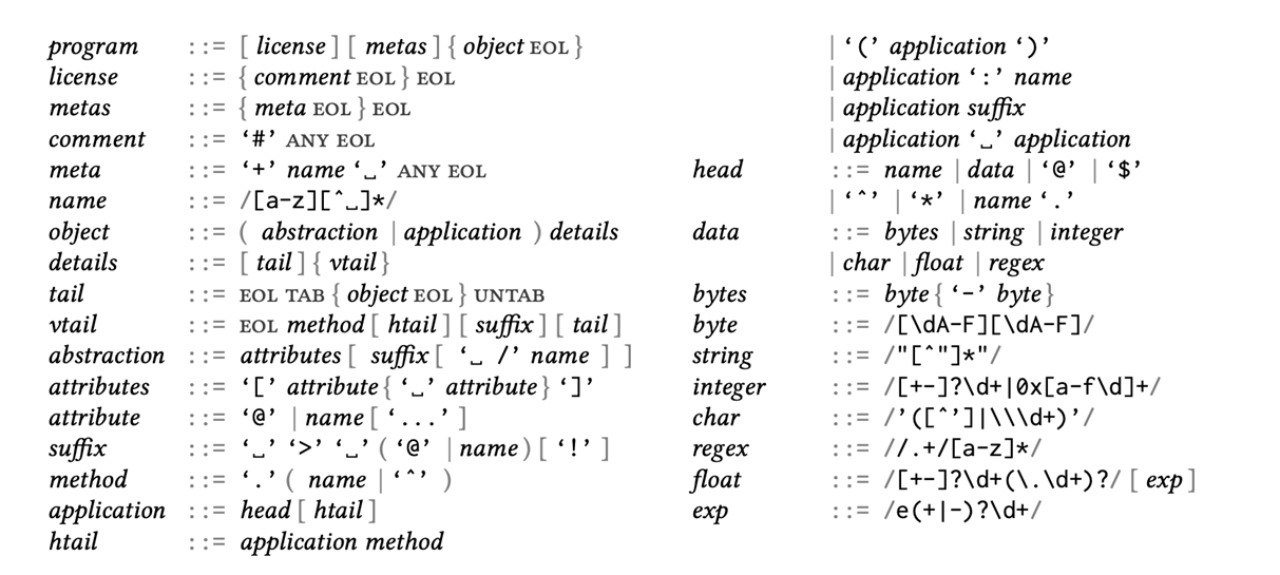
\includegraphics[width=1\textwidth,]{EOsyntxax.jpg}
  \caption{EO syntax}
  \label{fig:uml1}
\end{figure*}


\chapter{Basics}

\section{Hello,world!}
Create new file \ff{lab1.eo} in sandbox folder, and enter the code below:

\begin{ffcode}
+alias stdout org.eolang.io.stdout

[args...] > lab1
  stdout > @
    "Hello, world!"
\end{ffcode}

It is important to remember that each EO program must be ended with a new line without any symbols.


\section{Data Type Objects}

The EO Programming Language and The EO Standard Object Collection defines these data type objects: \texttt{bytes}, \texttt{bool}, \texttt{int}, \texttt{float}, \texttt{string}. All of them have \texttt{as-bytes} attribute, which is an abstraction of their representation as a sequence of bytes.
All primitives also have \texttt{as-hash} attribute, which, being an \texttt{int}, is their own implementation of a hash function. They also have \texttt{eq} attribute, which is \texttt{TRUE} if the primitive is equal to another object, through the use of \texttt{ˆ.as-bytes.eq}

\section{bytes Data Type Object}
The \texttt{bytes} data type object represents an abstraction of an sequence of bytes and can be empty or contain an theoretically unlimited number of bytes.
Fully Qualified Name: \texttt{org.eolang.bytes} (no aliasing or FQN reference required since the object is automatically imported).

\subsection{Syntax}
The \texttt{bytes} data type object may be parsed by the EO compiler directly from the source code. The syntax rules for \texttt{bytes} values are as follows.
EBNF Notation:
\begin{ffcode}
    BYTES   ::= BYTE ( ‘-’ BYTE ) | ‘--’
    BYTE    ::= [0-9A-F][0-9A-F]
\end{ffcode}

Example
\begin{ffcode}
+package sandbox
+alias stdout org.eolang.io.stdout
+alias sprintf org.eolang.txt.sprintf

[args...] > app
  stdout > @
    sprintf
      "%d\n"
      FF-FF-FF-FF-FF-FF-FF-FF.as-int
    
Running

IN$: ./run.sh
OUT>: -1
IN$: 
\end{ffcode}

\subsection{bytes Attributes}

\subsubsection{as-\textit{type} Attribute}
The object \texttt{bytes} has these four attributes, to turn itself into one of four primitive data objects: \texttt{as-int}, \texttt{as-bool}, \texttt{as-float}, and \texttt{as-string}. 
The attribute \texttt{as-int} expects the size of the sequence to be less or equal to eight. The attribute \texttt{as-bool} is \texttt{FALSE} only if all bytes equal to zero. The attribute \texttt{as-float} expects exactly eight bytes.

Example
\begin{ffcode}
+package sandbox
+alias stdout org.eolang.io.stdout
+alias org.eolang.txt.sprintf

[args...] > app
  stdout > @
    sprintf
      "%d\n%b\n%f\n%s\n"
      FF-FF-FF-FF-FF-FF-FF-FF.as-int
      00-.as-bool
      3F-80-00-00-00-00-00-00.as-float
      41-.as-string
    
Running

IN$: ./run.sh
OUT>: -1
OUT>: false
OUT>: 0.007813
OUT>: A
IN$: 
\end{ffcode}

\subsubsection{eq Attribute}
The \texttt{eq} attribute object is used for testing if two bytes objects are equal. The \texttt{eq} attribute object has one free attribute of type \texttt{bytes} that is the second object (the first object is the base object of the \texttt{eq} attribute).
If the \texttt{eq} attribute object is applied, it represents the result of the equality test (either true (if the objects are equal) or false (otherwise)).

Example
\begin{ffcode}
+package sandbox
+alias stdout org.eolang.io.stdout
+alias org.eolang.txt.sprintf

[args...] > app
stdout > @
  sprintf
    "%b"
    eq.
     FF-FF-FF-FE
     FF-FF-FF-FF

Running

IN$: ./run.sh
OUT>: false
IN$: 
\end{ffcode}

\subsubsection{and, or, xor Attributes}
Attributes objects \texttt{and}, \texttt{or}, \texttt{xor} are used for the bitwise operation of the same name. These attributes objects has one free attribute of type \texttt{bytes} that is the second object (the first object is the base object of these attributes).

Example
\begin{ffcode}
+package sandbox
+alias stdout org.eolang.io.stdout
+alias org.eolang.txt.sprintf

[args...] > app
  stdout > @
    sprintf
      "%b\n%b\n%b\n"
      eq.
        FF-.and 00-
        00-
      eq.
        FF-.or 00-
        FF-
      eq.
        FF-.xor FF-
        00-
    
Running

IN$: ./run.sh
OUT>: true
OUT>: true
OUT>: true
IN$: 
\end{ffcode}

\subsubsection{not Attributes}
The \texttt{not} attribute object is used for the bitwise operation of the same name. This attribute object has no free attributes.

Example
\begin{ffcode}
+package sandbox
+alias stdout org.eolang.io.stdout
+alias org.eolang.txt.sprintf
    
[args...] > app
  stdout > @
    sprintf
      "%b\n%b\n%b\n"
      eq.
        FF-.not
        00-
    
Running
    
IN$: ./run.sh
OUT>: true
IN$: 
\end{ffcode}

\subsubsection{left, right Attributes}
Attributes objects \texttt{left}, \texttt{right} are used for left and right bitwise shift. This attributes objects has one free attribute of type \texttt{int} that is the second object (the first object is the base object of these attributes). This free attribute specifies how many bits to shift.

Example
\begin{ffcode}
+package sandbox
+alias stdout org.eolang.io.stdout
+alias org.eolang.txt.sprintf

[args...] > app
  stdout > @
    sprintf
      "%b\n%b\n"
      eq.
        02-.left 2
        08-
      eq.
        10-.right 3
        02-
    
Running
    
IN$: ./run.sh
OUT>: true
OUT>: true
IN$: 
\end{ffcode}

\subsubsection{size Attribute}
The \texttt{size} attribute object is used to find out the total number of bytes in the bytes sequence. This attribute object has no free attributes.

Example
\begin{ffcode}
+package sandbox
+alias stdout org.eolang.io.stdout
+alias org.eolang.txt.sprintf

[args...] > app
  stdout > @
    sprintf
      "%d\n"
      FF-FF-F0.size
    
Running

IN$: ./run.sh
OUT>: 3
IN$: 
\end{ffcode}

\subsubsection{slice Attribute}
The \texttt{slice} attribute object is used to represents a bytes sub-sequence inside the current one. This attribute object has two free attributes of type \texttt{int}. The first attribute is the number of the element from which the sub-sequence starts, the second - at which the sub-sequence ends (included)

Example
\begin{ffcode}
+package sandbox
+alias stdout org.eolang.io.stdout
+alias org.eolang.txt.sprintf

[args...] > app
  stdout > @
    sprintf
      "%s\n"
      as-string.
        (FF-41-42-43-FF-FF.slice 1 3)
    
Running

IN$: ./run.sh
OUT>: ABC
IN$: 
\end{ffcode}

\subsubsection{concat Attribute}
The \texttt{concat} attribute object is used to make a new sequence, which is a concatenation of two byte sequences: the current and the provided one. This attribute object has one free attribute of type \texttt{bytes}. This free attribute provides a sequence of bytes to concatenate.

Example
\begin{ffcode}
+package sandbox
+alias stdout org.eolang.io.stdout
+alias org.eolang.txt.sprintf

[args...] > app
  stdout > @
    sprintf
      "%s\n"
      as-string.
        41-42.concat 43-44


Running

IN$: ./run.sh
OUT>: ABCD
IN$: 
\end{ffcode}

\section{bool Data Type Object}
The bool data type object represents a boolean value (either true or false) that can be used for performing logical operations.
Fully Qualified Name: org.eolang.bool (no aliasing or CFQN reference required since the object is automatically imported).

\subsection{Syntax}
The bool data type object may be parsed by the EO compiler directly from the source code. The syntax rules for bool values are as follows.
EBNF Notation

\begin{ffcode}
BOOL     ::= 'TRUE'
           | 'FALSE'
\end{ffcode}

Example
\begin{ffcode}
+package sandbox
+alias sprintf org.eolang.txt.sprintf
+alias stdout org.eolang.io.stdout

[args...] > app
  stdout > @
    sprintf
      "%b\n%b\n"
      TREU
      FALSE

Running

IN$: ./run.sh
OUT>: true
OUT>: false
IN$: 
\end{ffcode}

\subsection{bool Attributes}

\subsubsection{if Attribute}
The if attribute object is used for value substitution based on a condition that can be evaluated as a bool object.
The if attribute object has two free attributes:

\texttt{t} for the substitution if the base bool object is true.
\texttt{f} for the substitution if the base bool object is false.
If the if attribute object is fully applied, it represents the corresponding substitution value.

Example
\begin{ffcode}
+package sandbox
+alias sprintf org.eolang.txt.sprintf
+alias stdout org.eolang.io.stdout

[args...] > app
  stdout > @
    sprintf
      "%s\n%s\n%s\nThe max(2, 5) is: %d\n"
      TRUE.if
        "the first value is true"
        "the first value is false"
      FALSE.if
        "the second value is true"
        "the second value is false"
      if.
        2.lt 3
        "2 is less than 3"
        "2 is not less than 3"
      (5.lt 2).if
        2
        5

Running

IN$: ./run.sh
OUT>: the first value is true
OUT>: the second value is false
OUT>: 2 is less than 3
OUT>: The max(2, 5) is: 5
IN$: 
\end{ffcode}

\subsubsection{not Attribute}
The not attribute object represents a bool object with the inversed inner value of its base bool object.
The not attribute object has no free attributes.

Example
In this example, all the answers from the previous example (the if attribute section) are inversed with the not attribute.

\begin{ffcode}
+package sandbox
+alias sprintf org.eolang.txt.sprintf
+alias stdout org.eolang.io.stdout

[args...] > app
  stdout > @
    sprintf
      "[NOT Edition (all the answers are inversed with
      .not)]\n%s\n%s\n%s\nThe max(2, 5) is: %d\n"
      TRUE.not.if
        "the first value is true"
        "the first value is false"
      FALSE.not.if
        "the second value is true"
        "the second value is false"
      if.
        (2.lt 3).not
        "2 is less than 3"
        "2 is not less than 3"
      (5.lt 2).not.if
        2
        5

Running

IN$: ./run.sh
OUT>: [NOT Edition (all the answers are inversed with
.not)]
OUT>: the first value is false
OUT>: the second value is true
OUT>: 2 is not less than 3
OUT>: The max(2, 5) is: 2
IN$: 
\end{ffcode}

\subsubsection{and Attribute}
The and attribute object represents logical conjunction on a variety of bool objects.
The and attribute object has one free attribute x for the bool objects (conjuncts). x may be empty or may have any number of bool objects.

If the and attribute object is applied, it represents the conjunction of the base bool object and all the objects bound to the x attribute.

Example
\begin{ffcode}
+package sandbox
+alias sprintf org.eolang.txt.sprintf
+alias stdout org.eolang.io.stdout

[args...] > app
  TRUE > a
  TRUE > b
  TRUE > c
  FALSE > d
  stdout > @
    sprintf
      "a && b = %b\na && b && c = %b\na && b 
      && c && d = %b\n"
      a.and b
      a.and b c
      and.
        a
        b
        c
        d

Running

IN$: ./run.sh
OUT>: a && b = true
OUT>: a && b && c = true
OUT>: a && b && c && d = false
IN$: 
\end{ffcode}

\subsubsection{or Attribute}
The or attribute object represents logical disjunction on a variety of bool objects.
The or attribute object has one free attribute x for the bool objects (disjuncts). x may be empty or may have any number of bool objects.

If the or attribute object is applied, it represents the disjunction of the base bool object and all the objects bound to the x attribute.

Example
\begin{ffcode}
+package sandbox
+alias sprintf org.eolang.txt.sprintf
+alias stdout org.eolang.io.stdout

[args...] > app
  TRUE > a
  TRUE > b
  TRUE > c
  FALSE > d
  stdout > @
    sprintf
      "a || b = %b\na || b || c = %b\na || b || c 
      || d = %b\n"
      a.or b
      a.or b c
      or.
        a
        b
        c
        d

Running

IN$: ./run.sh
OUT>: a || b = false
OUT>: a || b || c = false
OUT>: a || b || c || d = true
IN$: 
\end{ffcode}

\subsubsection{while Attribute}
The while attribute object is used to evaluate its f free attribute until the base bool object is not false.
The f attribute object must have the free attribute i (the current iteration of the while loop).
On dataization, the while attribute object evaluates to the number of iterations the loop took.
Since objects are immutable, the memory object should be used as the loop condition (i.e., the base bool object of the while attribute). Moreover, the memory object should be changed somehow inside the f, otherwise the while will evaluate infinitely.

Example
\begin{ffcode}
+package sandbox
+alias stdout org.eolang.io.stdout
+alias sprintf org.eolang.txt.sprintf

[args...] > app
  memory 0 > x
  seq > @
    while.
      x.lt 11
      [i]
        seq > @
          stdout
            sprintf "%d x %d x %d = %d\n"
              x
              x
              i
              x.times (x.times i)
          x.write
            x.plus 1
          
Here, the i attribute of the f iteration object is 
used to find the x^3. However, the i attribute may 
stay unused inside the f.

Running

IN$: ./run.sh
OUT>: 0 x 0 x 0 = 0
OUT>: 1 x 1 x 1 = 1
OUT>: 2 x 2 x 2 = 8
OUT>: 3 x 3 x 3 = 27
OUT>: 4 x 4 x 4 = 64
OUT>: 5 x 5 x 5 = 125
OUT>: 6 x 6 x 6 = 216
OUT>: 7 x 7 x 7 = 343
OUT>: 8 x 8 x 8 = 512
OUT>: 9 x 9 x 9 = 729
OUT>: 10 x 10 x 10 = 1000
IN$: 
\end{ffcode}

\section{float Data Type Object}
The float data type object represents a double-precision 64-bit IEEE 754 floating-point number and can be used to perform various FPU computations.
Fully Qualified Name: org.eolang.float (no aliasing or FQN reference required since the object is automatically imported).

\subsection{Syntax}
The float data type object may be parsed by the EO compiler directly from the source code. The syntax rules for values are as follows.
EBNF Notation

\begin{ffcode}
FLOAT    ::= ( '+' | '-' )? [0-9]+ '.' [0-9]+
\end{ffcode}

Example
\begin{ffcode}
+package sandbox
+alias sprintf org.eolang.txt.sprintf
+alias stdout org.eolang.io.stdout

[args...] > app
  stdout > @
    sprintf
      "%f\n%f\n"
      1.5
      -3.71

Running

IN$: ./run.sh
OUT>: 1.500000
OUT>: -3.710000
IN$: 
\end{ffcode}

\subsection{eq Attribute}
The eq attribute object is used for testing if two float objects are equal.The eq attribute object has one free attribute x of type float that is the second object (the first object is the base object of the eq attribute).
If the eq attribute object is applied, it represents the result of the equality test (either true (if the objects are equal) or false (otherwise)).

Example
\begin{ffcode}
+package sandbox
+alias sprintf org.eolang.txt.sprintf
+alias stdout org.eolang.io.stdout

[args...] > app
  stdout > @
    sprintf
      "%b\n%b\n"
      1.5.eq 1.5
      -3.71.eq 3.71

Running

IN$: ./run.sh
OUT>: true
OUT>: false
IN$: 
\end{ffcode}

\section{string Data Type Object}
The string data type object represents a string literal.
Fully Qualified Name: org.eolang.string (no aliasing or FQN reference required since the object is automatically imported).

\subsection{Syntax}
The string data type object may be parsed by the EO compiler directly from the source code. The syntax rules for values are as follows.

EBNF Notation
\begin{ffcode}

STRING   ::= '"' ( '\"' | [^"] )* '"'
\end{ffcode}

Example
\begin{ffcode}
+package sandbox
+alias sprintf org.eolang.txt.sprintf
+alias stdout org.eolang.io.stdout

[args...] > app
  stdout > @
    sprintf
      "%s%s%s"
      "Hello, "
      "World! Welcome to The \"EO Docs\"!"
      "\n"

Running

IN$: ./run.sh
OUT>: Hello, World! Welcome to The "EO Docs"!
IN$: 
\end{ffcode}

Example
\begin{ffcode}
+package sandbox
+alias sprintf org.eolang.txt.sprintf
+alias stdout org.eolang.io.stdout

[args...] > app
  stdout > @
    sprintf
      "%b\n%b\n%b\n"
      "".eq ""
      "Hey".eq "Hey"
      "Hey".eq "hey"

Running

IN$: ./run.sh
OUT>: true
OUT>: true
OUT>: false
IN$: 
\end{ffcode}

\subsection{Additional Attributes For Working With strings}
The object org.eolang.txt.text is a decorator of org.eolang.string. So the text object contains methods for working with strings. Before using these methods, you need to make such an application:
\begin{ffcode}
(org.eolang.txt.text "String").trim
\end{ffcode}

\subsubsection{trim Attribute} 
The trim attribute object is used for trimming the base text object (i.e. trim is a string with whitespace removed from both ends of the base string).
The trim attribute object has no free attributes.
If the trim attribute object is applied (called), it represents the resulting trimmed string.

Example

\begin{ffcode}
+package sandbox
+alias sprintf org.eolang.txt.sprintf
+alias stdout org.eolang.io.stdout
+alias text org.eolang.txt.text

[args...] > app
  stdout > @
    sprintf
      "%s%s%s"
      trim.
        text "  Hello There  "
      trim.
        text "            !           "
      trim.
        text "\n"

Running

IN$: ./run.sh
OUT>: Hello There!IN$: 
Here, the \n escape sequence is trimmed as it is a
whitespace character.
\end{ffcode}

\subsubsection{as-int Attribute}
The as-int attribute object is used for parsing the base text object as an int object.
The format of the base text object must be as described below:

The first character of the string literal may be either + or -. This indicates the sign of the int value. The sign may be omitted (in such a case, the number is positive).
All the other characters of the string literal must be decimal digits (0-9).
If the format of the base string object is incorrect, the as-int attribute will fail on its application.
The as-int attribute object has no free attributes.
If the as-int attribute object is applied (called), it represents the parsed int object.

Example

\begin{ffcode}
+package sandbox
+alias sprintf org.eolang.txt.sprintf
+alias stdout org.eolang.io.stdout
+alias text org.eolang.txt.text

[args...] > app
  stdout > @
    sprintf
      "%d\n%d\n%d\n%d\n"
    as-int.
      text "1700"
    as-int.
      text "-1500"
    as-int.
      text "8"
    as-int.
      text "-0"

Running

IN$: ./run.sh
OUT>: 1700
OUT>: -1500
OUT>: 8
OUT>: 0
IN$: 
\end{ffcode}

\section{int Data Type Object}
The int data type object represents a 64-bit integer number.
Fully Qualified Name: org.eolang.int (no aliasing or FQN reference required since the object is automatically imported).

\subsection{Syntax}
The int data type object may be parsed by the EO compiler directly from the source code. The syntax rules for values are as follows.
EBNF Notation

\begin{ffcode}
INT      ::= ( '+' | '-' )? [0-9]+
\end{ffcode}
There is also an alternative syntax for hexadecimal numerals (i.e., with the base 16). This notation implies only non-negative values.

\begin{ffcode}
HEX      ::= '0x' [0-9a-f]+
\end{ffcode}


And an alternative notation for HEX integers:
The Int Data Type Railroad Diagram (HEX Notation)

Example
\begin{ffcode}
+package sandbox
+alias sprintf org.eolang.txt.sprintf
+alias stdout org.eolang.io.stdout

[args...] > app
  stdout > @
    sprintf
      "%d\n%d\n%d\n%#01x\n"
      -157
      1009283
      0xf.plus 1
      0xa

Running

IN$: ./run.sh
OUT>: -157
OUT>: 1009283
OUT>: 16
OUT>: 0xa
IN$: 
\end{ffcode}

Example
\begin{ffcode}
+package sandbox
+alias sprintf org.eolang.txt.sprintf
+alias stdout org.eolang.io.stdout
    
[args...] > app
  stdout > @
  sprintf
    "%b\n%b\n"
    eq.
      0xf
      15
    15.eq (0xf.plus 1)
    
Running

IN$: ./run.sh
OUT>: true
OUT>: false
IN$: 
\end{ffcode}

\subsection{int Attributes}

\subsubsection{lt Attribute}
The lt attribute object is used for testing if its base int object is less than its x free attribute (i.e. \$ $<$ x).
If the less attribute object is fully applied, it represents the result of the testing (either true (if the base object is less than x free attribute of the less) or false (otherwise)).

Example
\begin{ffcode}
+package sandbox
+alias sprintf org.eolang.txt.sprintf
+alias stdout org.eolang.io.stdout

[args...] > app
  stdout > @
    sprintf
      "%b\n%b\n"
      -7.lt 0
      lt.
        0
        0

Running

IN$: ./run.sh
OUT>: true
OUT>: false
IN$: 
\end{ffcode}

\subsubsection{plus Attribute}
The plus attribute object is used to calculate the sum of its base int object and the free attribute x of type int (i.e. \$+x).
If the plus attribute object is fully applied, it represents the resulting sum of the integer numbers.

Example
\begin{ffcode}
+package sandbox
+alias sprintf org.eolang.txt.sprintf
+alias stdout org.eolang.io.stdout

[args...] > app
  stdout > @
    sprintf
      "%d\n%d\n"
      plus.
        0x10
        16
      -16.plus 0x10

Running

IN$: ./run.sh
OUT>: 32
OUT>: 0
IN$: 
\end{ffcode}

\subsubsection{minus Attribute}
The minus attribute object is used to calculate the difference between its base int object and the free attribute x of type int (i.e. \$-x).
If the minus attribute object is fully applied, it represents the resulting difference of the integer numbers.

Example
\begin{ffcode}
+package sandbox
+alias sprintf org.eolang.txt.sprintf
+alias stdout org.eolang.io.stdout

[args...] > app
  stdout > @
    sprintf
      "%d\n%d\n"
      minus.
        0x10
        16
      -16.minus 0x10

Running

IN$: ./run.sh
OUT>: 0
OUT>: -32
IN$: 
\end{ffcode}

\subsubsection{neg Attribute}
The neg attribute object is used to negate its base int object (i.e. -\$).
If the neg attribute object is applied (called), it represents the resulting negation of the base int object.

Example
\begin{ffcode}
+package sandbox
+alias sprintf org.eolang.txt.sprintf
+alias stdout org.eolang.io.stdout

[args...] > app
  stdout > @
    sprintf
      "%d\n%d\n%d\n%d\n"
      5.neg
      0x10.neg
      (17.plus 3).neg
      17.neg.plus 3

Running

IN$: ./run.sh
OUT>: -5
OUT>: -16
OUT>: -20
OUT>: -14
IN$: 
\end{ffcode}

\subsubsection{times Attribute}
The times attribute object is used to calculate the product of its base int object and the free attribute x of type int (i.e. \$ × x).
If the times attribute object is fully applied, it represents the resulting product of the integer numbers.

Example
\begin{ffcode}
+package sandbox
+alias sprintf org.eolang.txt.sprintf
+alias stdout org.eolang.io.stdout

[args...] > app
  stdout > @
    sprintf
      "%d\n%d\n%d\n%d\n%d\n"
      -7.times 0
      13.times 1
      times.
        0x10
        0x10
      ((10.times 10).times 10).times 10
      10.times 10.times 10.times 10

Running

IN$: ./run.sh
OUT>: 0
OUT>: 13
OUT>: 256
OUT>: 10000
OUT>: 10000
IN$: 
\end{ffcode}

\subsubsection{div Attribute}
Example
\begin{ffcode}
+package sandbox
+alias sprintf org.eolang.txt.sprintf
+alias stdout org.eolang.io.stdout

[args...] > app
  stdout > @
    sprintf
      "%d\n"
      10.div 2

Running

IN$: ./run.sh
OUT>: 5
IN$: 
\end{ffcode}

\subsection{Additional Attributes For Working With int Objects}
The object org.eolang.math.number is a decorator of org.eolang.int. So the number object contains methods for working with int data type objects. Before using these methods, you need to make such an application:
\begin{ffcode}
(org.eolang.math.number 2).mod 1
\end{ffcode}

\subsubsection{mod Attribute}
The mod attribute object is used to calculate the floor remainder of the integer division of its base number object by the x free attribute (i.e. \$ fmod x).
If the mod attribute object is fully applied, it represents the resulting floor modulus (remainder).
The modulus for x = 0 is undefined. The resulting floor modulus has the same sign as the divisor x.
The relationship between the mod and div operations is as follows:
(x div y) * y + x mod y == x

Example
\begin{ffcode}
+package sandbox
+alias sprintf org.eolang.txt.sprintf
+alias stdout org.eolang.io.stdout
+alias number org.eolang.math.number

[args...] > app
  stdout > @
    sprintf
      "%d\n%d\n%d\n%d\n%d\n%d\n"
      (number 2).mod 1
      (number 7).mod 5
      (number 113).mod 10
      (number 113).mod -10
      (number -113).mod 10
      (number -113).mod -10

Running

IN$: ./run.sh
OUT>: 0
OUT>: 2
OUT>: 3
OUT>: 3
OUT>: -3
OUT>: -3
IN$: 
\end{ffcode}

\subsubsection{pow Attribute}
The pow attribute object is used to calculate the power of its base number object and the free attribute x of type int (i.e. \$\textasciicircum x).
If the pow attribute object is fully applied, it represents the resulting power of the base int object raised to the power of the x attribute.

Example
\begin{ffcode}
+package sandbox
+alias sprintf org.eolang.txt.sprintf
+alias stdout org.eolang.io.stdout
+alias number org.eolang.math.number

[args...] > app
  stdout > @
    sprintf
      "%d\n%d\n%d\n%d\n%d\n"
      (number 2).pow 10
      (number -2).pow 3
      (number 2).pow -10
      (number 2).pow 0
      (number 2).pow 1

Running

IN$: ./run.sh
OUT>: 1024
OUT>: -8
OUT>: 0
OUT>: 1
OUT>: 2
IN$: 
\end{ffcode}
Here, 2\textasciicircum(-10) results in 0 as well as raising all the integer numbers (except 0) to the negative power (-1, -2, -3, ...).s

\section{char Data Type Object}
\noindent\fbox{%
    \parbox{\textwidth}{%
        \textbf{Note:}
        The char object is not implemented yet, hence the char cannot be used for now.
    }%
}


The char data type object represents a single character.

Fully Qualified Name: org.eolang.char (no aliasing or FQN reference required since the object is automatically imported).

\subsubsection{Syntax}
The char data type object may be parsed by the EO compiler directly from the source code. The syntax rules for values are as follows.
EBNF Notation

\begin{ffcode}
CHAR     ::= "'" [0-9a-zA-Z] "'"
\end{ffcode}

\section{Command Line Interface Output}
The EO Standard Object Collection contains two objects for the CLI output: sprintf for strings formatting and stdout for plain text output.

\subsection{Plain Text Output. stdout}
For plain text output, the stdout object is used.
Fully Qualified Name: org.eolang.io.stdout.

\subsubsection{Usage}
The stdout object has one free attribute text that should be bound to the text to print.
The object bound to the text attribute must be of string type.
The stdout does not put the End of Line character at the end of the output, so the \\n escape sequence should be used in case if such a behavior is needed.
For the complete list of escape sequences supported by stdout, see the corresponding section of the article.

Example 1. The Plain Old “Hello, World”
\begin{ffcode}
+package sandbox
+alias stdout org.eolang.io.stdout

[args...] > app
  (stdout "Hello, World!\n") > @
Running
IN$: ./run.sh
OUT>: Hello, World!
IN$: 
\end{ffcode}

Example 2. Print the First Word of the User's Input
\begin{ffcode}
+package sandbox
+alias stdout org.eolang.io.stdout

[args...] > app
  stdout > @
    at.
      args
      0
Running
IN$: ./run.sh Hello Bye Thanks Ok
OUT>: HelloIN$: 
\end{ffcode}

Note: here, the Hello is printed with no EOL character at the end of the line because of the absence of it in the user input.

\subsection{Formatting Strings. sprintf}
For strings formatting, the sprintf object is used.
String formatting is the process of data injection into the string, optionally applying format patterns to the data.
Fully Qualified Name: org.eolang.txt.sprintf.

\subsubsection{Usage}
The sprintf object has two free attributes:

format for the format string that describes the formatting of the resulting string.
args for the data being injected into the string. args may be empty or may have any number of objects. args must be consistent with the format (i.e., the number and the types (as well as their order) of the objects in the format and the args should be the same).
If the sprintf object is fully applied, it represents the resulting formatted string.
For the format syntax reference, see this article.

Example. Format 'Em All
\begin{ffcode}
+package sandbox
+alias sprintf org.eolang.txt.sprintf
+alias stdout org.eolang.io.stdout

[args...] > app
  sprintf > formatted_string
    "int: %d, bool: %b, string: %s\n"
    2
    (2.lt 0)
    "Hey"

  (stdout formatted_string) > @

Running
IN$: ./run.sh
OUT>: int: 2, bool: false, string: Hey
IN$: 
\end{ffcode}


\section{Arrays}
The EO Standard Object Collection contains the array object for working with arrays of objects.
Fully Qualified Name: org.eolang.array (no aliasing or FQN reference required since the object is automatically imported).

\subsection{array Attributes}

\subsubsection{at Attribute}
The at attribute object is used to retrieve an object stored at the position i of the base array object.
The position i must be within 0 and the length of the array inclusively.
When applied, the at attribute object represents the object stored at the position i of the base array object.

Example
\begin{ffcode}
+package sandbox
+alias sprintf org.eolang.txt.sprintf
+alias stdout org.eolang.io.stdout

[args...] > app
  stdout > @
    sprintf
      "%s\n%s\n"
      args.at 0
      args.at 1

\end{ffcode}

In this example, the args array is used that consists of the CLI parameters passed to the program.

Running
\begin{ffcode}
IN$: ./run.sh Hello, World!
OUT>: Hello,
OUT>: World!
IN$: 
\end{ffcode}

\subsubsection{with Attribute}
The with attribute object is used to append the x object at the end of the base array object.
When applied, the with attribute object represents the resulting array object with the x at the end of it.

\begin{ffcode}
Example
+package sandbox
+alias sprintf org.eolang.txt.sprintf
+alias stdout org.eolang.io.stdout

[args...] > app
  args.with "New Element!" > argsExtended
  stdout > @
    sprintf
      "%s\n%s\n%s\n"
      argsExtended.at 0
      argsExtended.at 1
      argsExtended.at 2

\end{ffcode}
In this example, the args array is used that consists of the CLI parameters passed to the program.

Running
\begin{ffcode}
IN$: ./run.sh Hello, World!
OUT>: Hello,
OUT>: World!
OUT>: New Element!
IN$: 
\end{ffcode}

\subsection{Additional Attributes For Working With arrays}

The object org.eolang.collections.list is a decorator of org.eolang.array. So the list object contains methods for working with arrays. Before using these methods, you need to make such an application:
\begin{ffcode}
    (org.eolang.collections.list array).is-empty
\end{ffcode}

\subsubsection{reduce Attribute}
The reduce attribute object is used to perform the reduction operation of its base list object. The reduction is a process of accumulating a set of objects into one aggregated object.
The reduce attribute object has two free attributes:

\texttt{a} for the initial value of the accumulator.
\texttt{f} for the object that represents the reduction function. It must have two free attributes:
The first attribute is the current value of the accumulator.
The second attribute is the current object of the array.
The \texttt{f} attribute object aggregates the objects of the array in the accumulator. Objects of the array arrive into the \texttt{f} in the order these objects are stored in the array.
When applied, the reduce attribute object represents the resulting reduced accumulator object.

Example
\begin{ffcode}
+package sandbox
+alias sprintf org.eolang.txt.sprintf
+alias stdout org.eolang.io.stdout
+alias list org.eolang.collections.list
+alias text org.eolang.txt.text

[args...] > app
  [accumulator current] > reduceFunction
    plus. > @
      accumulator
      (text current).as-int

  reduce. > sum
    list args
    0
    reduceFunction

  stdout > @
    sprintf
      "%d\n"
      sum
\end{ffcode}

In this example, the args array is used that consists of the CLI parameters passed to the program. The array of numbers passed into the program is reduced into the sum of its elements.

Running
\begin{ffcode}
IN$: ./run.sh 1 2 3 4 5
OUT>: 15
IN$: 
\end{ffcode}

\section{Sequencing Computations. seq}
The EO Standard Object Collection contains the seq object for sequencing computations.
The seq object has one free attribute steps that may have an arbitrary number of steps that will be evaluated one by one, from the beginning to the end in the sequential order.
The seq object starts the dataization process for each of the objects bound to the steps attribute of it.
On dataization, the seq object evaluates into the result of datazation of the last step.
Fully Qualified Name: org.eolang.seq (no aliasing or FQN reference required since the object is automatically imported).

Example
\begin{ffcode}
+package sandbox
+alias sprintf org.eolang.txt.sprintf
+alias stdout org.eolang.io.stdout

[args...] > app
  seq > @
    stdout "Hello\n"
    stdout "These objects\n"
    stdout "will be dataized\n"
    stdout "one by one, in sequential order\n"

Running
IN$: ./run.sh
OUT>: Hello
OUT>: These objects
OUT>: will be dataized
OUT>: one by one, in sequential order
IN$: 
\end{ffcode}

\section{Mutable Storage in Memory. memory}
The EO Standard Object Collection contains the memory object for mutable storage in RAM.
Fully Qualified Name: org.eolang.memory (no aliasing or FQN reference required since the object is automatically imported).
Usage To use the memory object, the following steps are needed:

Make a copy of the memory object and bound it to some attribute.
To put an object into the memory object, the write attribute object is used. It has the x free attribute that is the object to put into the memory. The write attribute evaluates to true on dataization.
To retrieve the object stored in the memory, dataization of the memory object is used.

Example
\begin{ffcode}
+package sandbox
+alias sprintf org.eolang.txt.sprintf
+alias stdout org.eolang.io.stdout

[args...] > app
  memory > m
  seq > @
    m.write 1
    m.write (m.plus 1)
    m.write (m.plus 1)
    m.write (m.plus 1)
    stdout (sprintf "%d\n" m)

Running
IN$: ./run.sh
OUT>: 4
IN$: 
\end{ffcode}

\section{Self-practice}
\subsection{Tasks}
\begin{enumerate}
    \item (Easy) Implement an object that sums elements of an int (or float) array. Use the reduce attribute object of the array object (i.e., list.reduce). 
    \item (Middle) Implement an object that finds the product of integers numbers in an array. The object must be recursive.
    \item (Middle+) Implement an object that finds conjunction of booleans in an array using array.reduce. The object must short-circuit. This means that the reduce object must not compute any sub-conjunctions when the result is obvious (=0). Hint: Instead, the reduce object must just pass the answer until the array is processed with no sub-computations.
    \item (Middle++) Implement an object that finds disjunction of booleans in an array. The object must be tail-recursive. Also, the object must short-circuit. This means that the object must not compute any sub-disjunctions when the result is obvious (=1). Hint: Instead, the object must just “return” the answer at that point.
    \item (Middle) Implement an object that concatenates strings in an array. Use list.reduce. Hint: use sprintf.
    \item (Middle) Given an array of float objects representing temperature values in Celsius. Implement an object that finds the corresponding array of temperature values in Fahrenheit. Use list.map. Hint: the formula is (x°C × 9.0/5.0) + 32.0 = y°F
    \item (Middle+) Given an array of ints. Implement an object that finds the first (in other words, the leftmost) minimum in the array. The object must return another object with two attributes: index and value. Use list.reduce.
    \item (Middle++) Given an array of ints and the minimum object from Task 7. Implement the removeAt object that removes the element at position index and returns the resulting array. Use list.reducei (make sure that you are using reducei, not reduce). 
    \item (Hard) Given an array of ints and objects minimum and removeAt from Tasks 7, 8. Implement the selection sorting algorithm. 
    \item  (Easy) Given an array of objects. Implement the reverse object that reverses the order of objects from a, b, c, d, …, x, y, z to z, y, x, …, c, b, a. The object must be recursive.
    \item (Hard) Make your own .reduce operation for arrays from scratch. Implement an object that performs the reduce operation over an array (contents of the array may be of any type). Use recursion or tail-recursion.
    \item (Hard) Make your own .map operation for arrays from scratch. Implement an object that performs the map operation over an array (contents of the array may be of any type). Use recursion or tail-recursion.
    \item (Hard+) Make your own .map operation for arrays from scratch. Implement an object that performs the map operation over an array (contents of the array may be of any type). Use your own .reduce operation from Task 12 or the standard array.reduce (the choice is up to you and does not matter). Do not use recursion of any kind! Use only the .reduce operation to implement .map! Hint: .reduce transforms arrays (N) to a sole value (1), that’s why it is referred to as N-to-1 transformation operation. But nothing stops us to consider the sole output value (1) as another array!
\end{enumerate}

\subsection{Tests}
\begin{enumerate}
    \item What elemental operation of the EO language may be used for object creation?
    \begin{enumerate}
        \item Abstraction. // Yes! Abstraction may be compared with class declaration in Java. However, EO has no classes. The object defined through abstraction is a real object that may be used. So, yes. Abstraction creates objects (and allows us to define the structure of the object). 
        \item Decoration. // No :( Decoration is used to compose objects. This means that the object A decorated by the object B inherits (or extends) B’s attributes and adds its own attributes (that may possibly hide/shadow the original attributes of B). 
        \item Dataization. // No! Even though the actual dataization algorithm may instantiate objects in the target environment (for instance, inside JVM), these are implementation details of a concrete EO compiler. The EO language is declarative. We can’t manage the actual process of execution of our programs. The operation of dataization is the only one we can’t control. It’s done by the EO environment based on some rules. 
        \item Application. Yes! We can create copies of objects through application. Also, we can bind values with free attributes thanks to this operation. However, we can’t define the structure of objects when we apply them. That’s the main and principal difference when comparing this operation to abstraction. 
    \end{enumerate}
    
    \item What list attributes are normally used to implement N-to-N transformations?
    \begin{enumerate}
        \item list.reduce.
        \item list.length.
        \item list.empty.
        \item list.map.
        \item list.reducei.
        \item list.mapi.
    \end{enumerate}
    
    \item What list attributes are normally used to implement N-to-1 transformations?
    \begin{enumerate}
        \item list.reduce.
        \item list.length.
        \item list.empty.
        \item list.map.
        \item list.reducei.
        \item list.mapi.
    \end{enumerate}
    
    \item (Tricky question). What list attributes may be possibly used to implement N-to-N transformations?
    \begin{enumerate}
        \item list.reduce.
        \item list.length.
        \item list.empty.
        \item list.map.
        \item list.reducei.
        \item list.mapi.
    \end{enumerate}
    
    \item (Tricky question). What list attributes may be possibly used to implement N-to-1 transformations? 
    \begin{enumerate}
        \item list.reduce.
        \item list.length.
        \item list.empty.
        \item list.map.
        \item list.reducei.
        \item list.mapi.
    \end{enumerate}
\end{enumerate}


\chapter{Comparison between EO,Java,Kotlin,Groovy}
We tried to be as close to JVM languages as possible.
We examine next languages:

\section{Java}
The Java programming language originated as part of a research project to develop advanced software for a wide variety of network devices and embedded systems. The goal was to develop a small, reliable, portable, distributed, real-time operating platform. When the project started, C++ was the language of choice. But over time the difficulties encountered with C++ grew to the point where the problems could best be addressed by creating an entirely new language platform. Design and architecture decisions drew from a variety of languages such as Eiffel, SmallTalk, Objective C, and Cedar/Mesa. The result is a language platform that has proven ideal for developing secure, distributed, network-based end-user applications in environments ranging from network-embedded devices to the World-Wide Web and the desktop. 

\section{Kotlin}
Kotlin was designed to run on the JVM. It comes with its own compiler that compiles kotlin code to byte-code that can run on the JVM. The byte-code generated by kotlin compiler is equivalent to the byte-code generated by the Java compiler. Whenever two-byte code files run on JVM, due to their equivalent nature they can communicate with each other and that’s how interoperability is established in kotlin for Java . Kotlin was developed keeping interoperability in mind. A Kotlin class or a function can refer to the Java classes and their methods in a simple way. Kotlin program files (.kt) and Java program files (.java) can be in the same project. They are all compiled and converted to .class files which are byte-codes.

\section{Groovy}
Groovy is a dynamic and optionally typed object oriented scripting language. Just like Kotlin and Scala, groovy is interoperates well with Java; almost all Java code are also valid Groovy code.

\section{Abstraction}

\subsection{EO}
Already exists. The object abstracts behavior
(or cohesion)  of other objects.

LOC:
\begin{ffcode}
[x a b c] > polynomial 
  (((x.pow 2).times a).plus (x.times b)).plus c > @
  
\end{ffcode}
\subsection{Java}
To create an abstract class, just use the abstract 
keyword before the class keyword,
in the class declaration.

LOC
\begin{ffcode}
class Polynomial {
    public Polynomial
    (int x, int a, int b, int c){
    this.x=x;  
    this.a=a; 
    this.b=b;
    this.c=c;
    }
    public int compute() {
        return x*x*a + x*b + c;}
    }
}
\end{ffcode}
\subsection{Groovy}
To create an abstract class, just use the abstract 
keyword before the class keyword,
in the class declaration.

LOC
\begin{ffcode}
class Polynomial {
    public Polynomial
    (int x, int a, int b, int c){
    this.x=x;  
    this.a=a; 
    this.b=b;
    this.c=c;
    }

public int compute() {
    return x*x*a + x*b + c;}
    }
    
\end{ffcode}

\subsection{Kotlin}
Like Java, abstract keyword is used to declare abstract classes in Kotlin.
An abstract class cannot be instantiated (you cannot create objects of an abstract class). 
However, you can inherit sub-classes from can them.

\section{Encapsulation}

\subsection{EO}
Doesn't exist and will not be introduced

\subsection{Java}
Encapsulation in Java is a mechanism of wrapping 
the data (variables) and code acting on the 
data (methods) together as a single unit.
In encapsulation, the variables of a class will be
hidden from other classes, and can be accessed
only through the methods of their current class. 
Therefore, it is also known as data hiding.

\subsection{Groovy}
In Groovy, everything is public. There’s no idea 
of private fields or methods. At least, not in the way
they would be represented in C++ or Java.

\subsection{Kotlin}
OOP encapsulation in Kotlin unlike Python is enforced and has some fine grained levels (scope modifiers/keywords)

\section{Inheritance}

\subsection{EO}
Doesn't exist and won't be introduced.
The usual inheritance is presented by decorators (@)
The main idea is that in the production (inheritance couses 
many problems)

\subsection{Java}
In Java, it is possible to inherit attributes and methods from one class to another. We group the "inheritance concept" into two categories: 
\begin{itemize}
    \item sub-class (child) - the class that inherits from another class.
    \item super-class (parent) - the class being 
inherited from to inherit from a class, use the extends keyword.
\end{itemize}

\subsection{Groovy}
Inheritance can be defined as the process where one class acquires the properties (methods and fields) of another. With the use of inheritance the information is made 
manageable in a hierarchical order. The class which inherits the properties of other is known as subclass (derived class, child class) and the class whose  properties are inherited is known as super-class (base class, parent class). "extends" is the keyword used to inherit the properties of a class.

\subsection{Kotlin}
All classes in Kotlin have a common super-class Any, that is the default super-class for a class with no super-types declared. Any has three methods: equals(), hashCode() and toString(). Thus, they are defined for all Kotlin classes. By default, Kotlin classes are final: they can’t be inherited. To make a class inheritable, mark it with the open keyword.

\section{Polymorphism}

\subsection{EO}
Will be implemented (Ad hoc polymorphism)

Duck typing in computer programming is an application of the duck test —
"If it walks like a duck and it quacks like a duck, then it must be a duck
" — to determine whether 
an object can be used for a particular purpose. 
With normal typing, suitability is determined by an object's type.
 In duck typing, an object's suitability is determined by the presence 
of certain methods and properties, rather than the type of the object itself.

\subsection{Java}
Inheritance lets us inherit attributes and methods from another class.
 Polymorphism uses those methods to perform different tasks. 
This allows us to perform a single action in different ways.
 
\subsection{Groovy}
If you do this in Java (splitting the classes out to their own files of course), it won't compile. Java looks at the reference type for available methods, so you will get a NoSuchMethodException. In Groovy, however, it looks at the type of the object, not the type of the reference so the method is found at runtime.

\subsection{Kotlin}
Kotlin supports two forms of polymorphism because it is both strongly and statically typed. The first form of polymorphism happens when the code is compiled. The other form happens at runtime. Understanding both forms of polymorphism is critical when writing code in Kotlin.

\section{Data types}

\subsection{EO}
Presented like Atom Data Type. It is an acronym of "Access to Memory". It is a term used for simple numerical identifiers (other name is "handles") which represent some internal data structures in the system.

Moreover,object modeling/representation is used in different programming languages (Smalltalk, Oberon, Zonnon etc.). Function as an object model is commonly used in functional programming languages. Type inference in programming languages helps to deduce types

\subsection{Java}
Data types specify the different sizes and values that can be stored in the variable. 
There are two types of data types in Java:

Primitive data types: The primitive data types include Boolean, char, byte, short, 
int, long, float and double.
Non-primitive data types:
 The non-primitive data types include Classes, Interfaces and Arrays.

\subsection{Groovy}
Groovy supports the same number of primitive types as Java.

\subsection{Kotlin}
In Kotlin, everything is an object in the sense that we can call member functions and properties on any variable. 
Some of the types can have a special internal representation - for example, 
numbers, characters and boo leans can be represented 
as primitive values at runtime - but to the user they look like ordinary classes.

\chapter{SWOT about EO}
We compare Eolang efficiency to C++ and Java, discover the differences, identify pros and cons by SWOT analysis, define metrics for comparison, and write test cases as well as automate testing and bench-marking for the different EO compiler versions. The main goal is to analyze Eolang efficiency.

\section{Comparison Metrics}
\subsection{Criteria for comparison}
There are many criteria important to comparing or evaluating general purpose programming languages:

\begin{enumerate}
    \item \textbf{Simplicity of language constructs}.
    
The simplicity of a language design includes such measurable aspects as the minimality of required concepts and the integrity and consistency of its structures. Simpilicity here relates to ease of programming. Simple is beautiful is the golden mantra in programming. While efficiency and performance are major factors, simplicity and maintenance cost wins over them in many use cases. These become a deciding factor while choosing a programming language, exploring features in a language or even deciding on standard coding practices within an organization.

Binary result: yes/no.
    \item \textbf{Readability}.
    
Readability refers to the ease with which codes can be read and understood. This relates to maintainability, an important factor as many programs greatly outlive their expected lifetimes.

Binary result: yes/no.
    \item \textbf{Compilation speed}.
    
This metric identifies the program's total execution time(ms). This can comparatively help determine how long it takes to run an algorithm in different languages.

Result: 1..5, 5-high speed,1-low speed
    \item \textbf{Memory usage}.
    
The memory usage criteria identifies the  total amount of memory that were used due to program execution. Some programming languages may be efficient in memory consumption while others are not. This criteria is important for clarifying the differences between EO, C++ and Java.

Result: 1..5, 5-low usage,1-high usage.
    \item \textbf{LOC (Lines of code)}.
    
This refers to the total number of LOC that were used to develop a program. This metric is used to measure the size and complexity of a software project. It is measured by counting the number of lines in text of the program's source code. LOC can be used to predict the amount of effort that would be required to develop a program, as well as estimate programming productivity or maintainability once the software is developed.

Result:1..5, 5-high amount,1-low amount.
    \item \textbf{Debugging help}.
    
This criteria helps clarify the amount of tools and help available for the process of detecting and removing of existing and potential errors or bugs in a software code that can cause it to behave unexpectedly or crash.

Binary result: yes/no.
\end{enumerate}

In order to compare Eolang efficiency to C++ and Java and detect the differences, we select a number of algorithms to implement in all three languages. The following algorithms were chosen:
\begin{enumerate}
    \item Prim's algorithm
    \item Dijkstra's algorithm
    \item Kruskal's algorithm
    \item Ford-fulkerson's algorithm
\end{enumerate}

The justification for choosing these specific algorithms is that graph algorithms are usually complex, contain loops and recursive calls, and can be tested and compared based on different criteria. 

The test results of the implementation of these algorithms are capture under the following headings:

\begin{enumerate}
    \item vNum - the number of edges
    \item Time - the time of program execution
    \item Memory - the total memory used while program execution
\end{enumerate}

\subsection{Prim's algorithm}
Prim's algorithm is an algorithm for constructing the minimum spanning tree of a connected weighted undirected graph.

The input of the algorithm is a connected weighted undirected graph, which is represented by a sequence of integers separated by spaces.
Each group of 3 numbers describes an arc of the graph: the first two numbers are adjacent vertices, the third is the weight of the edge. 

Ex. 0 2 4 2 4 1 4 1 5 1 3 2 3 0 7

First, a random vertex is selected. The edge of the minimum weight incident to the selected vertex is searched for. This is the first edge of the spanning tree.
Next, an edge of the graph of the minimum weight is added to the tree in which only one of the vertices belongs to the tree.
When the number of tree edges is equal to the number of nodes in the graph minus one (the number of nodes in the graph and the tree are equal), the algorithm ends.

The result of the work of programs implementing the algorithm is a sequence of edges of the minimal spanning tree:
Ex. (2 4 - 1) (0 2 - 4) (4 1 - 5) (1 3 - 2)  

Time Complexity: O((V + E) log V)

\subsection{Dijkstra's algorithm}
Dijkstra’s algorithm is very similar to Prim’s algorithm for minimum spanning tree. Like Prim’s MST, we generate a SPT (shortest path tree) with a given source as a root. We maintain two sets, one set contains vertices included in the shortest-path tree, other set includes vertices not yet included in the shortest-path tree. At every step of the algorithm, we find a vertex that is in the other set (set of not yet included) and has a minimum distance from the source.
Below are the detailed steps used in Dijkstra’s algorithm to find the shortest path from a single source vertex to all other vertices in the given graph. 

Algorithm
\begin{enumerate}
    \item Create a set sptSet (shortest path tree set) that keeps track of vertices included in the shortest-path tree, i.e., whose minimum distance from the source is calculated and finalized. Initially, this set is empty. 
    \item Assign a distance value to all vertices in the input graph. Initialize all distance values as INFINITE. Assign distance value as 0 for the source vertex so that it is picked first. 
    \item While sptSet doesn’t include all vertices 
    
a) Pick a vertex u which is not there in sptSet and has a minimum distance value. 

b) Include u to sptSet. 

c) Update distance value of all adjacent vertices of u. To update the distance values, iterate through all adjacent vertices. For every adjacent vertex v, if the sum of distance value of u (from source) and weight of edge u-v, is less than the distance value of v, then update the distance value of v. 
\end{enumerate}

Time Complexity: O(E log V)

\subsection{Kruskal's algorithm}
The Kruskal's algorithm is used to find the minimum spanning tree of a graph. A minimum spanning tree (MST) or minimum weight spanning tree for a weighted, connected, undirected graph is a spanning tree with a weight less than or equal to the weight of every other spanning tree. The weight of a spanning tree is the sum of weights given to each edge of the spanning tree. A minimum spanning tree has (V – 1) edges where V is the number of vertices in the given graph.

To find the MST using the Kruskal's algorithm:
\begin{enumerate}
    \item Sort all the edges in non-decreasing order of their weight.
    \item (Union-Find algorithm) Pick the smallest edge. Check if it forms a cycle with the spanning tree formed so far. If cycle is not formed, include this edge. Else, discard it.
    \item Repeat step no. 2 until there are (V-1) edges in the spanning tree.
\end{enumerate}

Time Complexity: O(E log V)

\subsection{Ford-Falkerson Algorithm}
The Ford-Falkerson Algorithm is used to solve the maximum flow problem. This algorithm depends on the concept of residual graph.

To understand and implement it, let us first look at the concept of Residual Graph.

Residual Graph of a flow network is a graph which indicates additional possible flow. If there is a path from source to sink in residual graph, then it is possible to plus flow. Every edge of a residual graph has a value called residual capacity which is equal to original capacity of the edge minus current flow. Residual capacity is basically the current capacity of the edge. Let us now talk about implementation details. Residual capacity is 0 if there is no edge between two vertices of residual graph. We can initialize the residual graph as original graph as there is no initial flow and initially residual capacity is equal to original capacity. To find an augmenting path, we can either do a BFS or DFS of the residual graph. We have used DFS in below implementation. Using DFS, we can find out if there is a path from source to sink.

The important thing is, we need to update residual capacities in the residual graph. We subtract path flow from all edges along the path and we plus path flow along the reverse edges We need to plus path flow along reverse edges because may later need to send flow in reverse direction.

\subsubsection{Time Complexity:}
Time complexity of the above algorithm is O(max\_flow E).

\subsection{Comparison Metrics - \emph{Algorithms}}
\label{table:metrics}
\begin{center}
    \begin{tabular}{|p{0.1\linewidth}|p{0.25\linewidth}|l|}
\hline
Language&Metric&Grade \\ \hline
C++ &Simplicity &yes \\
Java &Simplicity &yes \\
EO &Simplicity &no \\ \hline
C++ &Readability &yes\\
Java &Readability &yes\\
EO &Readability &no\\\hline
C++ &Compilation speed&5(time:3 ms.)\\
Java &Compilation speed&4(time:1.18 s.)\\
EO &Compilation speed&1(time:30 s.)\\\hline
C++ &Memory usage&5(memory:30 mb.)\\
Java &Memory usage&3(memory:340 mb.)\\
EO &Memory usage&1(memory:2.96 gb.)\\\hline
C++ &LOC&5 (350 LOC)\\
Java &LOC&3 (500 LOC)\\
EO &LOC&1 (770 LOC)\\\hline
C++ &Debugging help&yes\\
Java &Debugging help&yes\\
EO &Debugging help&yes\\\hline
\end{tabular}
\end{center}


\section{SWOT Analysis}

The criteria listed above are equally important because they affect the development cost and effort required over the lifetime of the program, and also affect the usefulness and quality of the developed program.
It is important to note that several points are difficult to compare for several reasons, as far as various programming languages are concerned. One of the controversial points is that Eolang is generally positioned as a language intended for static code analysis, which, however, is not explicitly advertised and there is no special emphasis on this in the current project. However, this leads to the fact that initially, it is essentially a subject-oriented and not a universal language that does not allow effectively displaying not only the styles of writing programs but also having a much smaller set of expressive means for describing algorithms and data.

\subsection{STRENGTHS}
Here, in general, a fairly simple semantic model of the language can be noted, which is due to the initially laid down idea of forming an "elegant" programming style. Based on this, the program contains only objects, the semantics of which allows them to be used as actions (directives) that provide both a description of the functionality of algorithms and the structuring of data. This allows you to form a fairly compact \textbf{semantic model}, which is the strength of the language.

The solutions proposed in the language increase the reliability of the generated code, albeit often at the expense of efficiency. But for the main target of analysis and reliability improvement, this is not a significant factor.

When compared to C ++ and Java languages, it can be noted that in these languages there are many unreliable constructs for programming. The languages themselves have many redundant and overlapping constructs, which often do not allow the generation of unambiguous and reliable code.

\textbf{Compactness, extensibility and openness } can be used to describe the strength of Eolang.


\subsection{WEAKNESSES}
One of the weaknesses is that the limited capabilities of the language do not allow it to be used in many subject areas in comparison with C ++ and Java. That is, where high performance computing is required.

Another point to mention is \textbf{lack of tools} that provide support for parallel and distributed computing, which is currently used in one form or another in almost all modern programming languages.

And not enough attention is paid to the formation of the type system. Using a typeless solution can turn out to be unreliable in many situations, which, in turn, may lead to difficulties associated with static code analysis. In addition, in some cases, to increase control over data when writing programs in Eolang, additional constructions will have to be introduced to model data types and explicitly check them either during static analysis or at runtime.

For C++ and Java, static typing is used to control the data at compile time. In addition, these languages support dynamic typing due to Object-Oriented polymorphism and the possibility of dynamic type checking at runtime.

Currently, the EO community is limited. There are not many conferences, local meetups, forums, Facebook groups, open-source projects based on the language and people willing to help. 

Also, as mentioned in section \ref{table:metrics}, Eolang lacks \textbf{simplicity}. The EO language is barely simple to read and write and has a quite steep learning curve for new programmers. In comparison to the other languages in context, corresponding code in Eolang takes consumes more lines \textbf{(LOC)}. The comparison made in section \ref{table:metrics} shows that Eolang has minimal efficiency in terms of \textbf{memory consumption} and \textbf{compilation speed}. Thus, Eolang consumes a lot of resources, and increasing becomes complex as the code base gets large. These plus to the weaknesses of the language.

Lastly, conceptual incompleteness. The Eolang concept or idea is not fully or completely described.

\subsection{OPPORTUNITIES}
Most likely it is prudent to start with the possibilities since they determine the specifics of the language. The limitations through the OO paradigm and recursive computations based on the absence of object mutability possibly simplify the code for static analysis, but at the same time significantly reduces the number of effective techniques used in real programming. When creating algorithms, you often have to write longer and more inefficient code, which is difficult to further optimize when reduced to a real executor. At the same time, as the practice of using functional programming languages shows, the use of similar techniques increases the reliability of programs and ensures the formation of controlled code.

When comparing with C ++ and Java, it is enough to note here that both proposed languages are universal and include tools for writing programs that allow one to choose between reliable and efficient programming. In principle, it is possible to list these tools, emphasizing what is not in Eolang, emphasizing that this significantly expands the possibilities of programming, but often at the expense of the reliability of the code.

Also, the platform independence of Eolang provides an opportunity to potentially interoperate the language with many other languages and use existing libraries.

Additionally, there is potential \textbf{formalizability of semantics}, the presence of formal calculus of objects, the convergence of object and functional paradigms, potentially short and reliable code.

\subsection{THREATS}
Among the main threats, we could consider the use of the language not for its main purpose, which can lead to writing code that will be less expressive than the code written in C ++ and Java. At the same time, attempts to model the constructs of these languages in Eolang can lead to more cumbersome and less reliable code. In particular, explicit modeling of data types will require validation at runtime or may lead to the development of additional analysis programs to isolate and match data types during the static analysis phase.

It may also be worth noting the problem associated with the lack of type control when entering data when the incoming data in the presence of a \textbf{typeless} language model will be difficult to control. There are similar threats in other languages, but the presence of a static type system or explicit dynamic typing allows the ability to control the input and transformation of data directly using language constructs without additional modeling. Also, the typeless nature of the language drives it more in the direction of functional approach rather than OOP, as intended. It would be threatening to use Eolang as a system programming language since it lacks strong typing, compared to many system programming languages which rather are strongly typed to help manage complexity.

\chapter{Design patterns in EO}

\section{Background}
Design is one of the most difficult task in software development  and Developers, who have eagerly adopted them over the past years, needed to understand not only design patterns but the software systems before they can maintain them, even in cases where documentation and/or design models are missing or of a poor quality. In most cases only the source code as the basic form of documentation is available. Maintenance is a time-consuming activity within software development, and it requires a good understanding of the system in question. The knowledge about design patterns can help developers to understand the underlying architecture faster. Using design patterns is a widely accepted method to improve software development.
A design pattern is a general reusable solution to a commonly occurring  problem in software design. A design pattern isn't a finished design that can be transformed directly into code neither are they static entities, but evolving descriptions of best practices. It is a description or template for how to solve a problem that can be used in many different situations. A design pattern systematically names, motivates, and explains a general design that addresses a recurring design problem in object-oriented systems. It describes the problem, the solution, when to apply the solution, and its consequences. It also gives implementation hints.
Design patterns help to effectively speed up development and engineering processes by providing proven development patterns/paradigms. Quality software design requires considering issues that may not be visible until later in the implementation. Reusing design patterns helps to avoid subtle issues that may be catastrophic and help improve code reliability for programmers and architects familiar with the patterns. 
Design patterns provide general solutions, documented in a format that doesn't require specifics tied to a particular problem. They help software engineers to communicate using well-known, well understood names for software interactions. Common design patterns can be improved over time, making them more robust than ad-hoc designs. In short, the advantages of design patterns include decoupling a request from specific operations (Chain of Responsibility and Command), making a system independent from software and hardware platforms (Abstract Factory and Bridge), independent from algorithmic solutions (Iterator, Strategy, Visitor), or avoid modifying implementations (Adapter, Decorator, Visitor). Design patterns, overall, helps to thoroughly and designed well implemented frameworks enabling a degree of software reusability that can significantly improve software quality.


\section{Abstract Factory}
An abstract factory is a pattern that generates objects.

\subsubsection{Purpose}
Provides an interface for creating families of interconnected or interdependent objects without specifying their specific classes.

\subsubsection{Participants}
\begin{enumerate}
    \item AbstractFactory — abstract factory: declares an interface for operations that create abstract product objects.
    \item ConcreteFactory — specific factory: implements operations that create specific objects-products.
    \item AbstractProduct — abstract product: declares the interface for the type of object-product.
    \item ConcreteProduct — specific product: defines the product object created by the corresponding particular factory, and implements the AbstractProductinterface.
    \item Client: uses only interfaces that are declared in the AbstractFactory and  AbstractProduct classes.
\end{enumerate}

\subsubsection{Implementation}
\begin{ffcode}
1.	+package sandbox
2.	+alias stdout org.eolang.io.stdout
3.	+alias sprintf org.eolang.txt.sprintf
4.	
5.	[type] > abstractFactory
6.	  if. > concreteFactory
7.	    eq.
8.	      type
9.	      "1"
10.	    concreteFactory1
11.	    concreteFactory2
12.	
13.	  [] > createProductA
14.	    createProductA. > @
15.	      ^.concreteFactory
16.	  [] > createProductB
17.	    createProductB. > @
18.	      ^.concreteFactory
19.	
20.	[] > concreteFactory1
21.	  [] > createProductA
22.	    1 > @
23.	  [] > createProductB
24.	    2 > @
25.	
26.	[] > concreteFactory2
27.	  [] > createProductA
28.	    "one" > @
29.	  [] > createProductB
30.	    "two" > @
31.	
32.	[args...] > appAbstractFactory
33.	  abstractFactory > objFactory
34.	    args.at 0
35.	  stdout > @
36.	    sprintf
37.	      "ProductA: %s\nProductB: %s\n"
38.	      objFactory.createProductA
39.	      objFactory.createProductB 

\end{ffcode}


\textbf{Output}
\begin{ffcode}
$ ./run.sh 1
ProductA: 1
ProductB: 2
$ ./run.sh 2
ProductA: one
ProductB: two
\end{ffcode}


This program creates objects of integers or strings depending on the args parameter [0]. If  args[0] = 1, then objects 1 and 2 will be created, otherwise -  "one"  and  "two".
The template assumes the use of interfaces that are not present in the  EO. In this case, an attempt was made to implement the interface through the EO  object has a type parameter depending on which a specific implementation of the object factory is selected. This makes the interface object dependent on the set of implementations of this interface (when adding anew implementation, you must make changes to the interface object).

\section{Singleton (singles)}
A singleton is a pattern that generates objects.

\subsubsection{Purpose}
Ensures that the class has only one instance and provides a global access point to it.

\subsubsection{Participants}
Singleton Singleton:
\begin{enumerate}
    \item Defines an Instance operation that allows clients to access a single instance. Instance is a class operation,  that is,  a static method of a class
    \item May be responsible for creating your own unique instance.
\end{enumerate}

\subsubsection{Relations}
Clients access an instance of the Singleton class only through its Instance operation. 

\subsubsection{Implementation}
There are no classes in the EO, so this pattern is not implemented in its pure form. If we define Singleton in  terms  of  EO as an object that is guaranteed to have only one copy, then the implementation of this object is also impossible for the following reasons:
\begin{enumerate}
    \item There are no references in the EO.  Any use of an object in a location other than the place of definition is a copy of this object.
    \item EO  does not have the ability to restrict access to objects or prevent it from being copied. You cannot restrict the creation of copies of an object.

\end{enumerate}

\section{Prototype}
A prototype is a pattern that generates objects.

\subsubsection{Purpose}
Specifies the types of objects to create using the prototype instance and creates new objects by copying the prototype.


\begin{enumerate}
    \item — prototype: declares an interface for cloning itself.
    \item — Concrete Prototype: implements the operation of cloning itself.
    \item  — client: creates a new object by asking the prototype to clone itself.
\end{enumerate}

\subsubsection{Implementation}
In Eolang, each object can be copied, and each object can perform template functions.

\section{Observer}
In EO, all objects have immutable state. Based on the purpose of the template, its use in EO is pointless.

\section{Bridge}
A bridge is a pattern that structures objects.

\subsubsection{Purpose}
Separate abstraction from its implementation so that both can be changed independently.

\subsubsection{Participants}
\begin{enumerate}
    \item Abstraction — abstraction: defines the abstraction interface, and stores a reference to an object of type Implementor.
    \item RefinedAbstraction —  refined abstraction: extends the interface defined by abstraction.
    \item Implementor — implementer: defines the interface for the implementation classes. it does not have to exactly match the interface of the abstraction class. In fact both interfaces can be completely different. usually the interface of the Implementor class provides only primitive operations, and the  Abstraction class defines higher-level operations based on these primitives.
    \item ConcreteImplementor —  specific implementer: implements the interface of the Implementor class and defines its specific implementation.
\end{enumerate}

\subsubsection{Relations}
The Abstraction object redirects client requests to its  Implementor object.

\section{Chain of responsibility}
A chain of responsibilities is a pattern of behavior of objects.

\subsubsection{Purpose}
Avoids binding the sender of the request to its recipient by providing the ability to process the request to multiple objects. Binds the receiving objects to the chain and passes the request along that chain until it is processed.



\subsubsection{Participants}
\begin{enumerate}
    \item Handler —  handler: defines the interface for processing requests; (optionally) implements communication with the successor.
    \item ConcreteHandler — specific handler: processes the request for which it is responsible; Has access to his successor; If ConcreteHandler  is able to process the request, it does so, if it cannot, it sends it to its successor;
    \item Client: Sends a request to some ConcreteHandler object in the chain.
\end{enumerate}

\subsubsection{Relation}
A request initiated by a client is moved along the chain until some ConcreteHandler object takes responsibility for processing it.

\subsubsection{Implementation}
\begin{ffcode}
1.	+package sandbox
2.	+alias stdout org.eolang.io.stdout
3.	+alias sprintf org.eolang.txt.sprintf
4.	
5.	[nextHandler] > defaultHandler
6.	  [message] > process
7.	    "" > @
8.	
9.	[] > handler1
10.	  [message] > process
11.	    if. > @
12.	      message.eq "1"
13.	      "one"
14.	      ^.nextHandler.process message
15.	  defaultHandler > @
16.	    handler2
17.	
18.	[] > handler2
19.	  [message] > process
20.	    if. > @
21.	      message.eq "2"
22.	      "two"
23.	      ^.nextHandler.process message
24.	  defaultHandler > @
25.	    handler3
26.	
27.	[] > handler3
28.	  [message] > process
29.	    if. > @
30.	      message.eq "3"
31.	      "three"
32.	      ^.nextHandler.process message
33.	  defaultHandler > @
34.	    handler4
35.	
36.	[] > handler4
37.	  [message] > process
38.	    if. > @
39.	      message.eq "4"
40.	      "four"
41.	      ^.nextHandler.process message
42.	  defaultHandler > @
43.	    defaultHandler
44.	
45.	[args...] > appChain
46.	  handler1 > hChain
47.	  stdout > @
48.	    sprintf
49.	      "%s\n"
50.	      hChain.process
51.	        args.at 0 

\end{ffcode}


The input parameter args[0] is passed sequentially to 4 handlers, each of which processes its value (numbers from 1 to 4 are converted into words if another parameter is entered, an empty string is returned).

\section{Command}
Command pattern is a behavioral design pattern.

\subsubsection{Purpose}
Encapsulates a query in an object, thereby allowing clients to be parameterized  for different requests, queued or logged requests, and supports cancellation of operations.

\subsubsection{Participants}
\begin{enumerate}
    \item - Command — command: declares the interface to perform the operation.
    \item -	ConcreteCommand is a specific  team: defines the relationship between the Receiver receiving object and the action; implements the Execute operation by calling the corresponding operations of the  Receiverobject.
    \item — Client— client: Creates a ConcreteCommand class object and sets its recipient.
    \item - Invoker— initiator: calls the command to execute the request.
    \item - Receiver  — recipient: has information about how to perform the operations necessary to meet the request. Any class can act as a recipient.
\end{enumerate}

\subsubsection{Relations}
\begin{enumerate}
    \item - The client creates a ConcreteCommand object and sets a recipient for it.
    \item - The Invoker initiator saves the  ConcreteCommandobject.
    \item - The initiator sends a request by calling the ExecuteCommandOperation. If undoing of actions performed is supported, ConcreteCommand  stores sufficient status information to perform the cancellation before calling  Execute.
    \item - The ConcreteCommand  object  invokes the recipient's operations to execute the request.
\end{enumerate}

\section{Null}
The Null Object Pattern is one of the behavioral design patterns.

\subsubsection{Purpose}
Null object pattern is used to replace check of NULL object instance to simplify the use of dependencies that can be undefined.

\subsubsection{Problem}
In Null Object pattern, a null object replaces check of NULL object instance. Instead of putting if check for a null value, Null Object reflects a do-nothing relationship. Such Null object can also be used to provide default behaviour in case data is not available. The concept of null objects comes from the idea that some methods return null instead of real objects and may lead to having many checks for null in your code. 


In Java and C++, the key to the Null Object pattern is an abstract class that defines the interface for all objects of this type. The Null Object is implemented as a subclass of this abstract class. Because it conforms to the abstract class' interface, it can be used any place this type of object is needed. Null object should not have any state.


In Eolang, the concept of null does not exist as every object is meant to dataize to a value, and as such given a value on creation. As classes and interfaces do not exist here either, the closest implementation in Eolang would be to have every object implement a null attribute that either dataizes to a Boolean or a string representing a lack of value/data or whatever the default value of an object may be. In this case, there may still be checks to see if null is true or false or contains the expected string.

\subsubsection{Implementation}
\begin{ffcode}
1.	+package sandbox
2.	+alias stdout org.eolang.io.stdout
3.	+alias sprintf org.eolang.txt.sprintf
4.	+alias list org.eolang.collections.list
5.	
6.	[] > null
7.	  "null" > @
8.	
9.	[args...] > appNull
10.	  stdout > @
11.	    sprintf
12.	      "%s\n"
13.	      if.
14.	        (list args).is-empty
15.	        null
16.	        args.at 0 

\end{ffcode}

\textbf{Output:}
\begin{ffcode}
$ ./run.sh
null
\end{ffcode}

\section{Decorator}
Decorator is a structural design pattern.

\subsubsection{Purpose}
Decorator pattern allows you attach new behaviors to objects by placing these objects inside special wrapper objects that contain the behaviors.

\subsubsection{Problem}
Decorator pattern allows a user to add new functionality to an existing object without altering its structure. This pattern creates a decorator class which wraps the original class and provides additional functionality keeping class methods signature intact.


In Eolang, a copy of an object can be made, and new functionality be added. Here, the original object represents the decorator.

\subsubsection{Implementation}
\begin{ffcode}
1.	+package sandbox
2.	+alias stdout org.eolang.io.stdout
3.	+alias sprintf org.eolang.txt.sprintf
4.	+alias text org.eolang.txt.text
5.	
6.	[] > carsDecorate
7.	  8 > @
8.	
9.	[num] > someCars
10.	   decorateWithMoreCars num > @
11.	
12.	   [number] > decorateWithMoreCars
13.	     plus. > @
14.	       carsDecorate
15.	       number
16.	
17.	[args...] > appDecorator
18.	  stdout > @
19.	    sprintf
20.	      "%d\n"
21.	      someCars
22.	        as-int.
23.	          text (args.at 0)

\end{ffcode}

In this example, the object “someCars” increases the number of cars in decarDecorator is for itself.

\textbf{Output}

\begin{ffcode}
$ ./run.sh 5
13
\end{ffcode}

It can be concluded that decorator design pattern naturally exits in Eolang.

\section{Builder}
Suppose, we have a class with a variety of input parameters. The input parameters are used to configure instances of the class. Some of the parameters may be optional, while some of them are mandatory to be set up. Hence, the following techniques of configuration of instances of the class may be applied:
\begin{enumerate}
    \item Configuration of instance variables of an object directly in the user code through Setter Methods calls or by referencing variables straightforwardly. This practice may not be considered appropriate because it makes code instances more cohesive and interdependent while violating encapsulation of the inner state of objects (which may lead to breaking of the integrity of business logic of an application), and, hence, the usage of the practice is not encouraged. In addition, this technique may allow situations in which objects are being in an incomplete state, which also may break the logic of an application.
    \item Creation of subclasses of the considered class when each successor has a slightly changed prototype of its constructors. This technique implies that prototypes of constructors of different subclasses have subsets of optional parameters in them while omitting some parameters, which makes it possible to create configurable instances of objects in a controlled manner. This practice is more encouraged to be applied in practice since it implies control over the creational process. However, it is not recommended for use when choosing the sole parent superclass is challenging or when the practice produces a wide or deep hierarchy of inheritance
    \item Overloading of constructors or setting a single constructor with optional parameters. While this practice allows classes to create instances in a controlled way, it is undesirable in cases where the number of parameters or constructor overloads is too large to be manageable and understandable.
\end{enumerate}

The Builder pattern may be considered a universal solution to the problem. The pattern defines the Builder class, which has methods (stages) for building objects. The user code can call the stages in any order, omitting some of them (optional configurations). Also, the Builder class may check that all the required parameters are set up. At the end of construction, user code is required to call a method that finishes the construction process and returns a ready-made object. The pattern encapsulates the creational sensitive logic inside the Builder class and makes the configuration process manageable to the user code.

\subsubsection{Code Instances Involved}
Builder is an abstract class that defines the contract of the creational steps of Products for its successors (concrete builders). Also, the Builder superclass defines the finizaliotion method. 
Product is an interface for products (instances being created and configured through the Builder pattern). The interface defines the contract for all products so that these may be managed by Builders.
(optional) Director is a class, which defines higher-level (that is, higher than the level of "understanding" of the builder itself, for example, rules for mandatory fields and compliance with business logic) scripts for building objects. The director can be used to reuse some high-level business logic for constructing objects based on various builder implementations.

\subsubsection{Relations}
Implementations of the Product interface are products. Inheritors of the Builder class provide concrete implementations for the building steps (or borrow some of those steps from the superclass). The Director (optional entity) class can manage builders in a general style (based on some configuration) in accordance with the higher-level logic of business rules. The client code can contact the Director, giving it the configuration, or build an object using the Builder directly.

\subsubsection{Implementation}
First, we should mention that the problem solved by the Builder pattern may be addressed by the partial application mechanism embedded into the language as one of its features. The partial application mechanism allows programmers to partially apply objects (i.e., create objects with some or all of the input attributes omitted and then, optionally, set unbound attributes after throughout the program). This technique may be utilized as a more concise alternative to constructor overloading. Here is an example:
\begin{ffcode}
[a b c name] > triangle
  plus. > perimeter
    plus.
      a
      b
    c

  sprintf > toString
    "The triangle is named '%s'."
    name


[args...] > app
  triangle > triangleA
    10:a
  triangleA > triangleABC
    7:b
    8:c
  triangleABC > triangleABCNamed
   "My Triangle":name
  triangle > triangleNamed
    "My Another Triangle":name

\end{ffcode}


Here, we have the triangle object with input attributes a, b, c, and name. The triangle object has two bound attributes: perimeter (which relies on a, b, and c) and toString (which relies on name). Object app demonstrates the partial application mechanism. So, triangleA has only the a attribute bound, triangleABC has all the sides (a, b, c) sat up, triangleABCNamed has all the sides and its name configured, and triangleNamed has the name only. All three triangles are constructed through partial application (meaning, some of the attributes are left unbound or were bound after). The above example demonstrates an alternative solution to the problem of optional configuration of objects. However, this solution does not encapsulate the creation process of objects. Hence, the Builder pattern still may have its place in the EO environment.

Consider the following example:

\begin{ffcode}
[] > builder
  subbuilder triangle > @
  [triangleEntity] > subbuilder
    # finalizes the construction process
    [] > finalize
      ^.^.subbuilder > @
    # configures the a free attribute
    [aVal] > setA
      ^.^.subbuilder > @
        ^.^.triangleEntity
          (^.validateSide aVal):a
    # configures the b free attribute
    [bVal] > setB
      ^.^.subbuilder > @
        ^.^.triangleEntity
          (^.validateSide bVal):b
    # configures the c free attribute
    [cVal] > setC
      ^.^.subbuilder > @
        ^.^.triangleEntity
          (^.validateSide cVal):c
    # configures the name free attribute
    [nameVal] > setName
      ^.^.subbuilder > @
        ^.^.triangleEntity
          (^.validateName nameVal):name
    # validates side value
    [val] > validateSide
      if. > @
        val.greater 0
        val
        error
          "The side of a triangle must not 
          be less than 1!"
    # validates name
    [val] > validateName
      if. > @
        val.length.neq 0
        val
        error
          "The name of a triangle must not be empty!"

[args...] > app
  builder > b
  finalize. > triangleABC
    setC.
      setB.
        setA.
          builder
          10
        12
      0

\end{ffcode}


Here we implemented the principles of the Builder pattern through measures supplied by the EO language. The builder object contains the subbuilder attribute object that implements the construction steps (setA, setB, setC, setName) as well as validation sub-steps (validateSide, validateName) and the finalize attribute that finishes the construction process and returns the resulting object. Initially, the instantiation of the builder object is substituted with a copy of the subbuilder object with an empty (meaning, all free attributes are unbound) copy of the constructing object. On each construction step, the subbuilder object returns itself by passing a changed version of the constructing object to its constructor. The construction steps have validation substeps that may implement some complex business logic. Validation steps may return an error or a validated object, which may lead to an interruption of the program execution and prevent inconsistency of the business logic.
In conclusion, we would like to notice that the problem originally stated above (problem of optional configuration of objects with a lot of input parameters) and solved with the Builder pattern may not be actual to EO since it has the partial application mechanism that allows programmers to perform such configuration and, in addition, EO does not allow objects to have more than four free attributes (although, this restriction may be mitigated through passing complex object structures as free attributes). Nevertheless, the EO implementation of the Builder pattern may find its utilization in scopes where encapsulation of the creational process of objects is required. For instance, it may be needed when business logic validation of values passed for binding to free attributes is required.


\section{Factory Method}
The Factory Method Pattern is a creational object-oriented design pattern.

\subsubsection{Purpose}
Defines the creational method in the Creator superclass that defines a rule (that is, an interface or a contract) for creating an object (product) of some supertype Product. This method is used by the superclass or its more specific implementations, and the factory method can also be called from outside the class by other entities within the application. Concrete implementations of the Creator class with a factory method can return subtypes of the Product type, thereby "tailoring" a specific implementation of the product class to the one required by the factory method contract. Hence, the pattern allows programmers to implement seamless configuration of the architecture of the application.

\subsubsection{Problem}
The pattern addresses the problem of extending the architecture of an application. By specifying  the product contract (Product Interface) and by defining the class contract with the Factory Method Class, the architect separates the responsibility for creating the product itself from other methods of the creator class. This can be useful when:
\begin{enumerate}
    \item It is not known what types of the Product class may be used in the future, but it may be appropriate to leave a headroom for a potential extension of the application architecture. Otherwise, this can be interpreted as an implementation of the "Open / Closed” principle (O in SOLID).
    \item Implementation of the principle of "Single Responsibility" (S in SOLID). The code responsible for setting (configuring) a specific version of the product can be placed in a single place, for example, in a class that configures the application based on the environment settings. Here, the Dependency Injection mechanism can also be used to perform such a configuration in an invisible manner.
    \item The pattern allows programmers to separate the logic of product creation from other logic of the creator class. This facilitates the reuse of identical code.
\end{enumerate}


\subsubsection{Code Instances Involved}
Creator is an abstract class that defines the contract of the reutilized steps (here, it is someOperation) and the creational step (createProduct) of Products for its successors (concrete creators). 
Product is an interface for products (instances being created and configured through the Factory Method pattern). The interface defines the contract for all products so that these may be managed by the pattern.

\subsubsection{Relation}
Implementations of the Product interface are products. Inheritors of the Creator class provide concrete implementations for the creational method and inherit the rest methods. The concrete implementation of the creational method may return different implementations of Product, which implies the substitution of logic (or configurability of the application). 

\subsubsection{Implementation}
The EO programming language does not have interfaces, classes, and types. Because of it, we may omit defining the Product interface contract (since it would not impose any requirements). Consider the following implementation of the pattern in EO: 

\begin{ffcode}
[] > creator
  # left to be redefined
  [] > createObject
  # operation over products
  [] > performOperation
    createObject.getWeight.plus 1 > @

[] > concreteCreatorA
  creator > @
  [] > createObject
    productA > @

[] > concreteCreatorB
  creator > @
  [] > createObject
    productB > @

[] > productA
  # let's suppose that this implementation
  # gets value from the production server
  [] > getWeight
    42 > @

[] > productB
  # let's suppose that this implementation
  # gets value from the testing server
  [] > getWeight
          24 > @

\end{ffcode}

Here, we have the creator object with the performOperation attribute (the logic to be reused) and the createObject attribute (the logic to be redefined for flexible substitution of objects). The concreteCreatorA and concreteCreatorB objects have the creator object as their decoratee, so that these might inherit the reusable logic. Both objects define the createObject attribute that hides the original attribute of the same name from the decoration hierarchy. Objects productA and productB implement the attribute of interest (getWeight) differently. One of them may at the value from the production server, while another takes it from the testing environment. This example demonstrates the implementation of the classic version of the pattern in EO. However, we may consider a more EO-idiomatic example, free from additional structures (concrete creators) utilized in statically typed class-based object-oriented languages such as Java or C++. Consider the following example: 

\begin{ffcode}
[concreteCreator] > creator
  concreteCreator.createObject > createObject
  # operation over products
  [] > performOperation
    createObject.getWeight.plus 1 > @

[] > productA
  # let's suppose that this implementation
  # gets value from the production server
  [] > getWeight
    42 > @

[] > productB
  # let's suppose that this implementation
  # gets value from the testing server
  [] > getWeight
    24 > @

[args...] > app
  creator > creatorObject
    []
      [] > createObject
        if. > @
          (args.at 0).eq "test"
          productB
          productA

\end{ffcode}

Here, we used the technique of passing concreteCreator as a free attribute of the object creator. Its concreteCreator is passed in the app object. The decoratee has the only attribute createObject that the creator object inherits and relies on. The createObject attribute decides what version of a product should be chosen based on the environment configuration. This implementation of the pattern may be considered as more idiomatic and flexible from the EO perspective.


\section{The Closures Functional Programming Technique}
Since the EO programming language may be considered semi-functional, it might be useful to apply one of the widely adopted functional programming techniques, closures, in it. Simply put, the closures mechanism implies capturing outer lexical scope variables inside a function defined inside the scope with a consequent utilization of the function in other scopes. To support this technique, a language must operate over function as if they are first-class citizens (i.e., a language must return function or pass functions as parameters). Here is an example of this technique in JavaScript:

\begin{ffcode}
function makeAdder(x) {
  return function(y) {
    return x + y;
  };
}
var add5 = makeAdder(5);
var add10 = makeAdder(10);
console.log(add5(2));  // 7
console.log(add10(2)); // 12
\end{ffcode}

Here, we have the makeAdder function that returns an anonymous function capturing its outer state x. The state is then utilized when the returned function is applied with its own parameter y. In other words, the inner anonymous function remembers the value of x and uses it even when the actual value disappeared from the stack. This technique may be useful to emulate access modificators in functional languages: 

\begin{ffcode}
var counter = (function() {
  var privateCounter = 0;
  function changeBy(val) {
    privateCounter += val;
  }

  return {
    increment: function() {
      changeBy(1);
    },

    decrement: function() {
      changeBy(-1);
    },

    value: function() {
      return privateCounter;
    }
  };
})();

console.log(counter.value());  // 0.

counter.increment();
counter.increment();
console.log(counter.value());  // 2.

counter.decrement();
console.log(counter.value());  // 1.
\end{ffcode}

Here, the outer function counter returns a complex object-like structure containing functions that capture the state of the counter function. The state of the counter function is also complex: it has a mutable local variable privateCounter, and the changeBy function that mutates the value in the unified manner. The user code may not access the value and the mutating functions directly: both of them disappeared from the stack. However, the closures returned by the outer function still may do it. Hence, the technique allows functional programmers to simulate private state. 

We surely may reproduce the similar technique of capturing the lexical scope in EO:
\begin{ffcode}
[] > counter
  memory 0 > privateCounter
  [val] > changeBy
    privateCounter.write > @
      privateCounter.plus val
  [] > @
    [] > increment
      ^.changeBy 1 > @
    [] > decrement
      ^.changeBy (-1) > @
    [] > value
      ^.privateCounter > @

\end{ffcode}

\section{Summary about patterns}
It is possible to conclude that (1) EO is principally applicable to all the considered patterns; (2) For some patterns, EO is able to give a fairly concise and intuitively clear code, since the language combines the features of Functional Programming and OOP; (3) the issues of effective implementation of patterns on EO are largely determined by the characteristics of the environment (IDE + compiler) and today remain open.

Also, EO has no local variables or any kind of stack-lifetime storage. Instead, any name refers to an object (stored in heap) that may be accessed through the scope of any other object via the dot-notation mechanism. Even anonymous objects may allow programmers to access its local scope (including parent and decoration hierarchies) freely. In addition, EO has no access modification instruments. This makes closures technique almost similar to the partial application mechanism. Moreover, the publicity of any attribute of any object makes encapsulation impossible in the language. This differentiates EO from functional programming languages and, also, from object-oriented languages. Absence of instruments of access modification (or simulation of it) may be a severe violation of object-oriented principle of encapsulation, which may lead to insecure environments breaking business logic of problem domains.

EO is fundamentally applicable to all the patterns considered. 2) For some patterns, EO is able to give a fairly concise and intuitively clear code, since the language combines the features of Functional Program (FP) and OOP. 3) the issues of effective implementation of patterns on EO are largely determined by the characteristics of the environment (IDE + compiler).

\chapter{References}
\section{Opportunities}
JPeek : This module was built into the pipeline of the JPeek tool, which we now call, EO-JPeek.
\url{https://github.com/HSE-Eolang/eo-jpeek}

Algorithms implementation: ( Dijkstra; Prim; Kruskal; Ford-Falkerson ), is it possible to implement hard enough algorithms with EO? Would EO manage big enough input data? May EO code be functional and useful, yet idiomatic? We tried to address these questions in this work.
\url{https://github.com/polystat/eo-graphs}

Design Patterns: This is to help better assess the EO programming language and suggest alternatives of design patterns in EO that could replace such patterns which are not supported in the language. This repository contains descriptions and EO implementation of some popular software design patterns.
\url{https://github.com/HSE-Eolang/eodesignpatterns}

Simple Tutorial: With a help of this repository you will get familiar with EO programming. Moreover, this repository has the documentation on the language and its standard library.
\url{https://github.com/HSE-Eolang/eo_labs}


The EO sandbox with examples: This repository contains the examples of EO programs with description.
\url{https://github.com/cqfn/eo/tree/master/sandbox/hse}

\section{Contacts}
Hadi Saleh: 
\url{https://www.hse.ru/staff/hadisaleh}
mail: hsalekh@hse.ru


Alexander Legalov:
\url{https://www.hse.ru/org/persons/407667114}
mail: alegalov@hse.ru


Sergey Zykov:
\url{https://www.hse.ru/org/persons/3468544}
mail: szykov@hse.ru

Eugene Popov:
mail: gluttonous.pumpkin@gmail.com

Vitaliy Korzun:
mail: aventador3000@gmail.com

Joseph Attakorah 
mail: juxluvjoe@gmail.com
\end{document}
